% ==========================================================================
%  Sections 3, 4, 5 — Draft
%  Performance Modelling of CUDA Programs
%  Author: Parikshit Gehlaut
% ==========================================================================

% ------------------------------------------------------------------
% SECTION 3 — Background & Motivation
% ------------------------------------------------------------------

\section{Background \& Motivation}
\label{sec:background}

GPU performance models help programmers understand how fast their code can run
before they write it.
A good model takes a few numbers about the hardware and the workload,
and gives back a prediction of throughput.
In this section we review two such models: Volkov's three-bound formula
and Hong~\&~Kim's MWP/CWP framework.
We show why Volkov's model is the better choice for modern GPUs.

% ------------------------------------------------------------------
% 3.1  Volkov's Model
% ------------------------------------------------------------------
\subsection{Volkov's Model}
\label{subsec:volkov_model}

Volkov~\cite{volkov2016understanding} models GPU throughput as the minimum of
three bounds.
Given $n$ active warps per SM and arithmetic intensity $\alpha$ (compute
instructions per memory instruction), the throughput in warp-instructions
per cycle per SM is:
%
\begin{equation}
T_m \;=\; \min\!\Biggl(
  \underbrace{\frac{n}{mem_{lat} + \alpha \cdot alu_{lat}}}_{\text{latency bound}},\;\;
  \underbrace{mem_{thru}\vphantom{\frac{n}{1}}}_{\text{memory bound}},\;\;
  \underbrace{\frac{issue_{thru}}{\alpha + 1}}_{\text{issue bound}}
\Biggr)
\label{eq:volkov}
\end{equation}

Each bound captures a different bottleneck:

\begin{itemize}
  \item \textbf{Latency bound.}
    At low occupancy there are not enough warps to hide the latency of
    memory loads ($mem_{lat}$) and arithmetic operations ($alu_{lat}$).
    Throughput grows linearly with~$n$.

  \item \textbf{Memory bound.}
    The memory bus can only deliver $mem_{thru}$ warp-instructions per cycle
    per SM, no matter how many warps are active.
    This is the effective bandwidth ceiling.

  \item \textbf{Issue bound.}
    The instruction schedulers can issue at most $issue_{thru}$ warp-instructions
    per cycle per SM.
    When $\alpha$ is large, each warp contains many compute instructions that
    compete for issue slots.
\end{itemize}

The total predicted throughput in GFLOP/s is:
%
\begin{equation}
P \;=\; \underbrace{W \cdot N_{SM} \cdot f_{clock}}_{C} \;\cdot\; \alpha \;\cdot\; T_m
\label{eq:gflops}
\end{equation}
%
where $W = 32$ is the warp size, $N_{SM}$ is the number of SMs, and
$f_{clock}$ is the clock frequency in GHz.
The constant~$C$ converts from warp-operations per cycle per SM to GFLOP/s.

This model is useful because it is a single closed-form expression.
It needs only four hardware parameters ($mem_{lat}$, $alu_{lat}$,
$mem_{thru}$, $issue_{thru}$), has no scheduling heuristics,
and can be evaluated in a spreadsheet.


% ------------------------------------------------------------------
% 3.2  Hong & Kim (2009) — Limitations on Modern GPUs
% ------------------------------------------------------------------
\subsection{Hong \& Kim (2009) --- Limitations on Modern GPUs}
\label{subsec:hong_kim}

Hong and Kim~\cite{hong2009analytical} predict GPU performance using two
metrics: Memory Warp Parallelism (MWP) and Computation Warp Parallelism (CWP).
MWP counts how many memory requests from different warps can overlap at the
same time.
CWP counts how much computation fits into the time it takes for one memory
request to finish.
The model then picks one of three formulas depending on which
metric is larger.

The key limitation of this model is that it does not account for arithmetic
pipeline latency.
Hong and Kim treat computation time as the number of instructions multiplied by
the \emph{issue rate} (typically 1 cycle per instruction).
They do not include the pipeline depth of 4 cycles that real FP32 units need
to produce a result.
When arithmetic intensity is low, this does not matter much --- memory
latency dominates and both models give similar predictions.
But when arithmetic intensity is high, the missing $alu_{lat}$ term causes
Hong~\&~Kim's model to overestimate throughput because it thinks
the compute instructions finish faster than they actually do.

We show this in Figure~\ref{fig:hk_vs_volkov}.
At $\alpha = 32$, both models produce similar curves and both track the
measured data on RTX\,5000 (left pair).
At $\alpha = 64$, Hong~\&~Kim predict roughly 2$\times$ higher throughput
than what we measure, while Volkov's model stays close to the data (right pair).

\begin{figure}[t]
  \centering
  \begin{minipage}{0.48\linewidth}
    \centering
    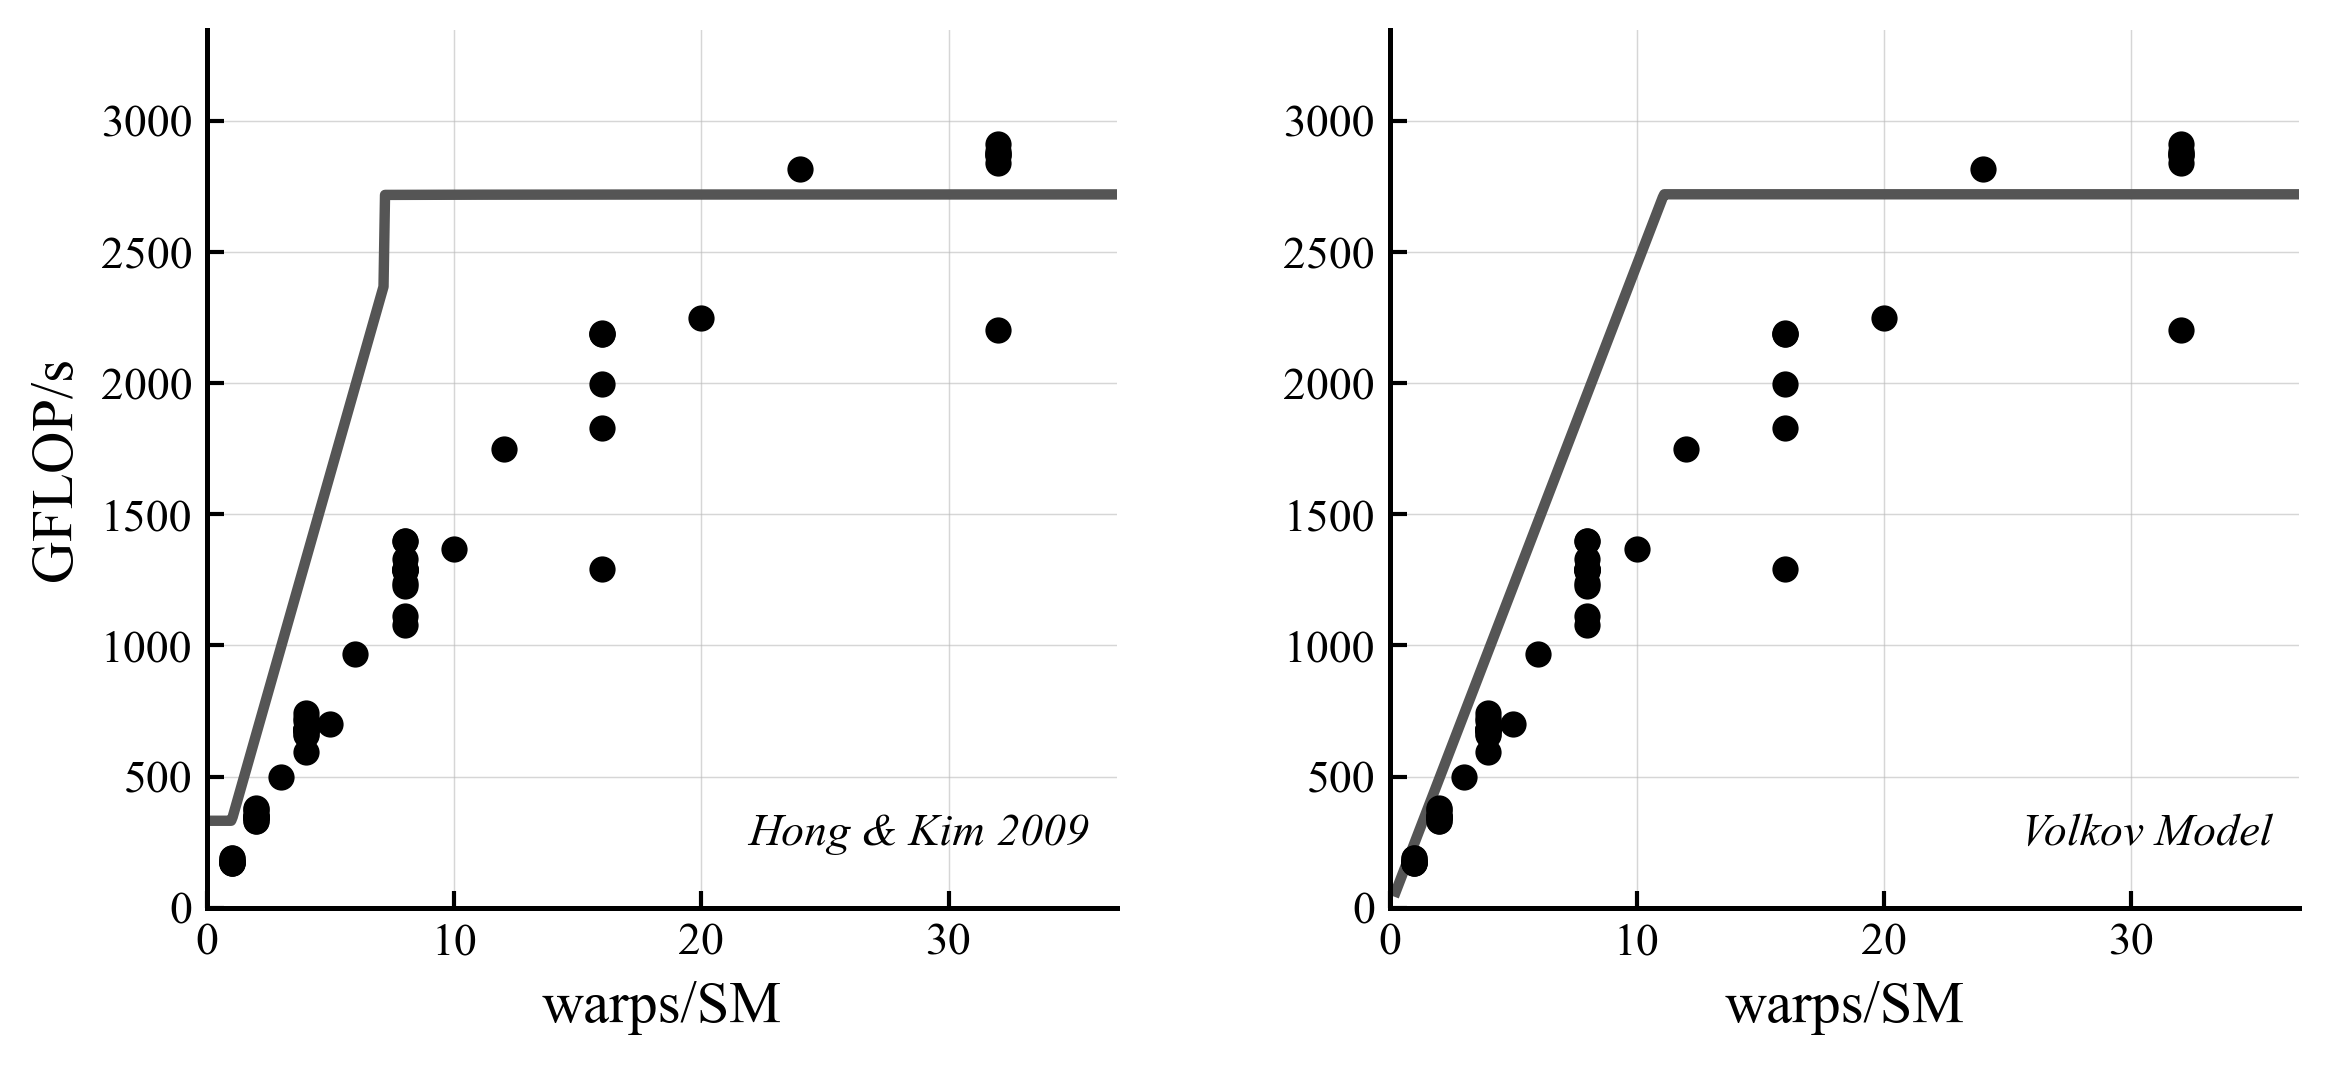
\includegraphics[width=\linewidth]{motivation/hk_vs_volkov_fixed_a32.png}
  \end{minipage}
  \hfill
  \begin{minipage}{0.48\linewidth}
    \centering
    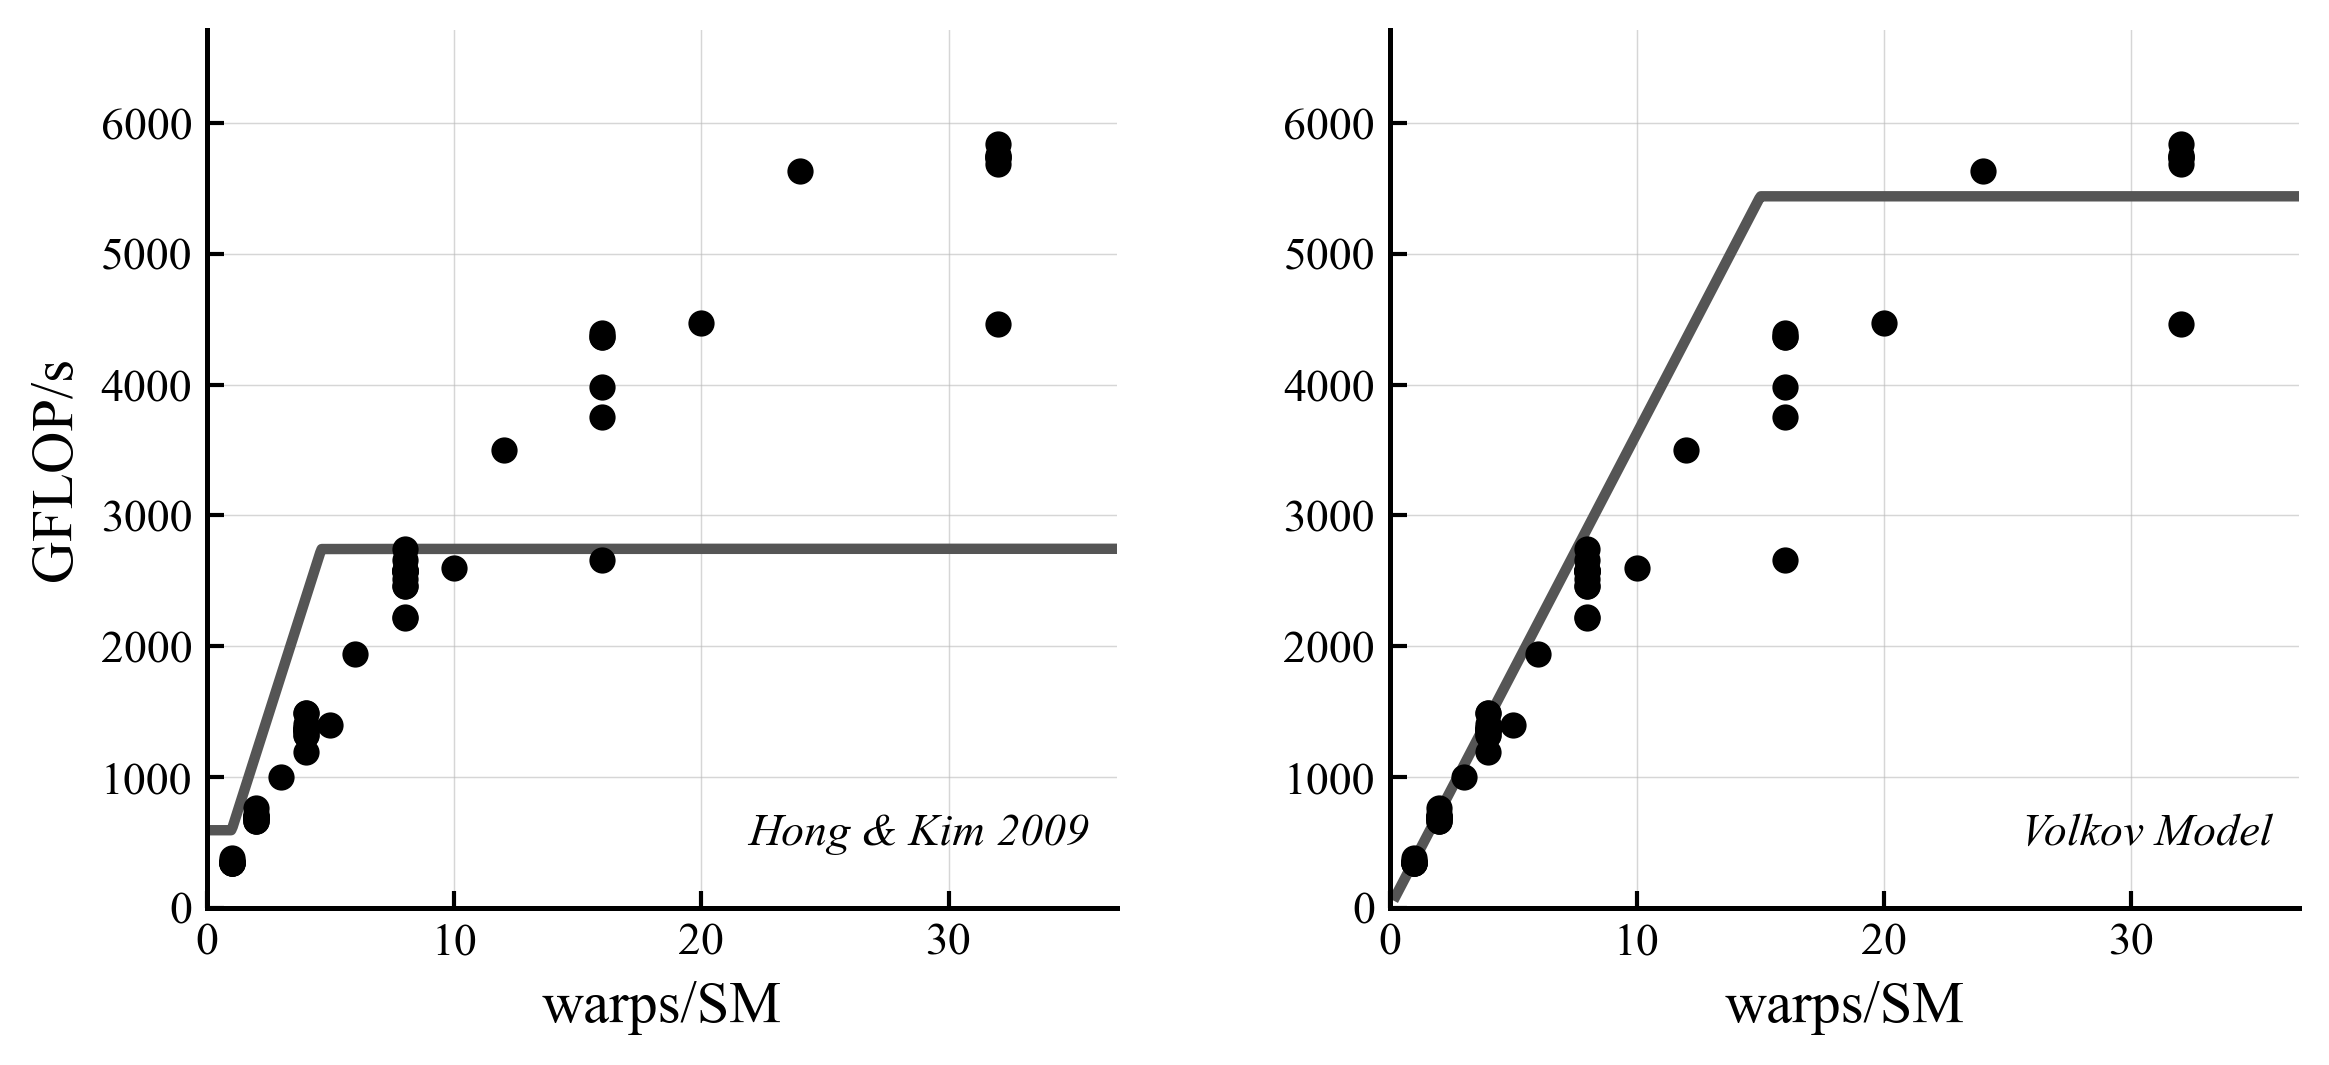
\includegraphics[width=\linewidth]{motivation/hk_vs_volkov_fixed_a64.png}
  \end{minipage}
  \caption{Hong~\&~Kim vs.\ Volkov on RTX\,5000.
    Left: $\alpha = 32$ --- both models agree with measured data.
    Right: $\alpha = 64$ --- Hong~\&~Kim overestimates throughput by
    $\approx 2\times$ because it ignores $alu_{lat}$.
    Black dots are measured GFLOP/s; grey curves are model predictions.}
  \label{fig:hk_vs_volkov}
\end{figure}

The lesson is clear:
Hong~\&~Kim's omission of $alu_{lat}$ causes a systematic error on modern GPUs
where the arithmetic pipeline depth (4 cycles) is large enough to become
a bottleneck at high arithmetic intensity.


% ------------------------------------------------------------------
% 3.3  Why Volkov's Model
% ------------------------------------------------------------------
\subsection{Why Volkov's Model}
\label{subsec:why_volkov}

Volkov's model captures all three bottlenecks --- latency, memory bandwidth,
and issue throughput --- in a single formula.
It treats $alu_{lat}$ as a first-class parameter, so it remains accurate at
high arithmetic intensity where Hong~\&~Kim breaks down.
Our evaluation (\S\ref{sec:evaluation}) confirms this on three modern GPUs:
Quadro RTX\,5000 (Turing), A100 (Ampere), and H100 (Hopper).

Other analytical models exist.
Baghsorkhi et al.~\cite{baghsorkhi2010adaptive} build a work-flow graph
to predict execution time, and Zhang and Owens~\cite{zhang2011quantitative}
extend Hong~\&~Kim's MWP/CWP approach with better memory modelling.
% TODO: co-author may expand this paragraph.
We choose Volkov's model for this study because of its simplicity and
because it directly connects hardware parameters to throughput
without requiring per-kernel program analysis.


% ------------------------------------------------------------------
% SECTION 4 — Design & Methodology
% ------------------------------------------------------------------

\section{Design \& Methodology}
\label{sec:design}


% ------------------------------------------------------------------
% 4.1  Parameter Measurement Methodology
% ------------------------------------------------------------------
\subsection{Parameter Measurement Methodology}
\label{subsec:param_measurement}

Volkov's model needs four parameters.
We measure three of them ($mem_{lat}$, $alu_{lat}$, $mem_{thru}$) using custom
CUDA microkernels and derive the fourth ($issue_{thru}$) from the
architecture specification.
All microkernels use 4-byte (\texttt{uint32\_t}) loads, matching Volkov's
original methodology.
Each warp load moves $32 \times 4 = 128$~bytes.


% ---- mem_lat ----
\paragraph{Memory Latency ($mem_{lat}$).}
The unloaded latency of a global memory load in clock cycles.
We measure it with \texttt{mem\_lat\_kernel.cu}, which runs a
\emph{pointer-chasing} loop: each 4-byte load produces the index for the
next load, forming a chain that the compiler cannot reorder.
Algorithm~\ref{alg:mem_lat} shows the key loop:
\texttt{curr\_idx = d\_indices[curr\_idx]}.
We use \texttt{\#pragma unroll 1} to stop the compiler from unrolling, so the
loop has exactly one load per iteration with instruction-level parallelism of~1.

We sweep all combinations of threads per block
(TPB $\in \{32, 64, 128, 256, 512\}$) and shared memory per block
(SHMEM $\in \{0, 4, 8, \ldots, 96\}$~KB) to vary occupancy.
At each point we record both mean and minimum warp latency.
We take the minimum observed latency across all configurations as $mem_{lat}$,
because that value reflects the hardware latency without contention.

\begin{algorithm}[t]
\caption{Memory Latency Microkernel}
\label{alg:mem_lat}
\begin{algorithmic}[1]
\STATE \textbf{Input:} \texttt{d\_indices[]} (uint32\_t array), \texttt{start\_indices[]}, \texttt{iterations}
\STATE \textbf{Shared Mem:} \texttt{shmem[]} \COMMENT{Occupancy control}
\STATE \texttt{curr\_idx} $\leftarrow$ \texttt{start\_indices[global\_tid]}
\STATE Record \texttt{start\_clock}
\STATE \textbf{Pragma Unroll 1} \COMMENT{Force serialisation}
\FOR{$i = 0$ \textbf{to} \texttt{iterations}}
    \STATE \texttt{curr\_idx} $\leftarrow$ \texttt{d\_indices[curr\_idx]} \COMMENT{4-byte dependent load}
\ENDFOR
\STATE Record \texttt{end\_clock}
\STATE \texttt{latency} $\leftarrow$ (\texttt{end\_clock} $-$ \texttt{start\_clock}) / \texttt{iterations}
\end{algorithmic}
\end{algorithm}


% ---- alu_lat ----
\paragraph{Arithmetic Latency ($alu_{lat}$).}
The pipeline latency of a single floating-point instruction in clock cycles.
We measure it with \texttt{alu\_lat\_kernel.cu}, which runs a dependent chain
of register-to-register operations: \texttt{c = c + a} (FADD),
\texttt{c = c * a} (FMUL), or \texttt{c = fma(a, b, c)} (FMA).
Each result feeds into the next instruction, so the chain cannot overlap.
The inner loop is unrolled by a factor of~32 to reduce loop overhead.

Algorithm~\ref{alg:alu_lat} shows the structure.
We sweep the same TPB and SHMEM combinations as for memory latency.
At low occupancy the pipeline is uncontested and we see the true pipeline depth.
At high occupancy, contention inflates the measured latency above the structural
floor.

\begin{algorithm}[t]
\caption{Arithmetic Latency Microkernel (FADD / FMUL / FMA)}
\label{alg:alu_lat}
\begin{algorithmic}[1]
\STATE \textbf{Register:} \texttt{volatile float c} $\leftarrow$ \texttt{lane\_id} $\times$ 0.1
\STATE \textbf{Register:} \texttt{volatile float a} $\leftarrow$ 1.000001
\STATE Record \texttt{start\_clock}
\FOR{$i = 0$ \textbf{to} \texttt{outer\_iterations}}
    \STATE \textbf{Pragma Unroll 32}
    \FOR{$j = 0$ \textbf{to} 32}
        \STATE \texttt{c} $\leftarrow$ \texttt{c + a} \COMMENT{or \texttt{c * a}, or \texttt{fma(a, b, c)}}
    \ENDFOR
\ENDFOR
\STATE Record \texttt{end\_clock}
\STATE Sink \texttt{c} to shared memory \COMMENT{Prevent optimisation}
\STATE \texttt{latency} $\leftarrow$ (\texttt{end\_clock} $-$ \texttt{start\_clock}) / (\texttt{outer\_iters} $\times$ 32)
\end{algorithmic}
\end{algorithm}


% ---- mem_thru ----
\paragraph{Peak Memory Throughput ($mem_{thru}$).}
The maximum rate at which memory instructions retire, in warp-instructions
per cycle per SM.
We measure it with \texttt{mem\_thru\_kernel.cu}, which streams through a
512~MB array of \texttt{uint32\_t} indices using coalesced, linear loads.
We use 1024~blocks of 256~threads to saturate the memory bus.
The kernel reports GB/s, and we convert to $mem_{thru}$ as:
%
\begin{equation}
mem_{thru} = \frac{\text{BW (GB/s)}}{f_{clock} \;\cdot\; N_{SM} \;\cdot\; 128\;\text{bytes/warp-instr}}
\label{eq:mem_thru}
\end{equation}
%
The denominator uses 128~bytes because each warp-instruction loads
$32 \times 4 = 128$~bytes.


% ---- issue_thru ----
\paragraph{Issue Throughput ($issue_{thru}$).}
The maximum number of warp-instructions the schedulers can issue per cycle
per SM.
We derive this from the GPU architecture:
each SM has 4 sub-partitions, each with one warp scheduler.
On Turing and Ampere, each sub-partition has 16 FP32 cores, so a 32-thread
warp takes 2 cycles to issue, giving 0.5 warp-instr/cycle per scheduler
and $issue_{thru} = 4 \times 0.5 = 2.0$.
On Hopper, each sub-partition has 32 FP32 cores, so a warp issues in 1 cycle
and $issue_{thru} = 4 \times 1.0 = 4.0$.


% ------------------------------------------------------------------
% 4.2  Model Initialisation
% ------------------------------------------------------------------
\subsection{Model Initialisation}
\label{subsec:model_init}

We run the microkernels on three GPUs: Quadro RTX\,5000 (Turing),
A100 (Ampere), and H100 (Hopper).
Table~\ref{tab:params} lists the measured parameters.
The coefficient $C = W \times N_{SM} \times f_{clock}$
converts per-SM throughput to GFLOP/s.

\begin{table}[t]
  \centering
  \caption{Measured model parameters for all three GPUs.
    $mem_{lat}$ and $alu_{lat}$ are in clock cycles;
    $mem_{thru}$ and $issue_{thru}$ are in warp-instr/cycle/SM.}
  \label{tab:params}
  \begin{tabular}{lrrr}
    \toprule
    \textbf{Parameter} & \textbf{RTX\,5000} & \textbf{A100} & \textbf{H100} \\
    \midrule
    $mem_{lat}$ (cycles)        & 236   & 240   & 352   \\
    $alu_{lat}$ (cycles)        & 4     & 4     & 4     \\
    $mem_{thru}$ (warp-instr/cy/SM) & 0.0305 & 0.0205 & 0.0220 \\
    $issue_{thru}$ (warp-instr/cy/SM) & 2.0 & 2.0 & 4.0 \\
    \midrule
    $C$ (GFLOP/s at $T_m = 1$) & 2787.84 & 6142.56 & 6408.96 \\
    \bottomrule
  \end{tabular}
\end{table}

The full throughput model for each GPU is then:
%
\begin{equation}
P = C \;\cdot\; \alpha \;\cdot\; \min\!\biggl(
  \frac{n}{mem_{lat} + \alpha \cdot alu_{lat}},\;
  mem_{thru},\;
  \frac{issue_{thru}}{\alpha + 1}
\biggr)
\label{eq:full_model}
\end{equation}

Table~\ref{tab:expressions} shows the fully expanded expression for each GPU.

\begin{table}[t]
  \centering
  \caption{Instantiated throughput expressions for all three GPUs.}
  \label{tab:expressions}
  \begin{tabular}{|l|p{7.0cm}|}
    \hline
    \textbf{GPU} & \textbf{Predicted GFLOP/s} \\
    \hline
    RTX\,5000 &
    $2787.84 \;\cdot\; \alpha \;\cdot\;
    \min\!\bigl(\frac{n}{236 + 4\alpha},\;
    0.0305,\;
    \frac{2.0}{\alpha+1}\bigr)$ \\[6pt]
    \hline
    A100 &
    $6142.56 \;\cdot\; \alpha \;\cdot\;
    \min\!\bigl(\frac{n}{240 + 4\alpha},\;
    0.0205,\;
    \frac{2.0}{\alpha+1}\bigr)$ \\[6pt]
    \hline
    H100 &
    $6408.96 \;\cdot\; \alpha \;\cdot\;
    \min\!\bigl(\frac{n}{352 + 4\alpha},\;
    0.0220,\;
    \frac{4.0}{\alpha+1}\bigr)$ \\[6pt]
    \hline
  \end{tabular}
\end{table}


% ------------------------------------------------------------------
% 4.3  Running Example — RTX 5000 (α = 32)
% ------------------------------------------------------------------
\subsection{Running Example: RTX\,5000 at $\alpha = 32$}
\label{subsec:running_example}

We walk through the three bounds of Equation~\ref{eq:full_model} for
RTX\,5000 with $\alpha = 32$:

\begin{enumerate}
  \item \textbf{Latency bound:}
    $n / (236 + 32 \times 4) = n / 364$.
    At $n = 1$ warp this gives $T_m = 0.00275$;
    at $n = 32$ warps it gives $T_m = 0.0879$.
    Throughput grows linearly until it hits one of the other bounds.

  \item \textbf{Memory bound:}
    $mem_{thru} = 0.0305$.
    This is constant and does not depend on $n$.
    The latency bound crosses this ceiling at $n \approx 364 \times 0.0305 \approx 11.1$~warps.

  \item \textbf{Issue bound:}
    $issue_{thru} / (\alpha + 1) = 2.0 / 33 = 0.0606$.
    This is higher than $mem_{thru}$, so for this $\alpha$ value the
    memory bound is tighter than the issue bound.
    The issue bound only becomes active at higher $\alpha$ values.
\end{enumerate}

Below $\approx 11$ warps/SM, the workload is latency-limited: adding more warps
helps.
Above $\approx 11$ warps/SM, the memory bus is saturated and more warps do not
help.
The issue bound at 0.0606 is above the memory bound, so it never activates.
The model predicts a peak throughput of
$2787.84 \times 32 \times 0.0305 = 2720$~GFLOP/s,
and the measured peak on RTX\,5000 at $\alpha = 32$ is $\approx 2875$~GFLOP/s.


% ------------------------------------------------------------------
% 4.4  Workload: Synthetic Streaming Kernel
% ------------------------------------------------------------------
\subsection{Workload: Synthetic Streaming Kernel}
\label{subsec:synthetic_kernel}

To test the model we need a workload with controllable arithmetic intensity
and measurable occupancy.
We use a synthetic kernel (\texttt{synthetic\_kernel\_streaming.cu}) that
matches Volkov's original experimental setup.

Each loop iteration does:
\begin{enumerate}
  \item One 4-byte dependent load: \texttt{curr\_idx = d\_indices[curr\_idx]}.
  \item Reinterpret the loaded index as a float: \texttt{tmp = int\_as\_float(curr\_idx)}.
  \item $\alpha$ dependent FMUL operations: \texttt{tmp = tmp * 1.0f}, repeated
        $\alpha$ times.
  \item Reinterpret the float back to an index: \texttt{curr\_idx = float\_as\_int(tmp)}.
\end{enumerate}

Algorithm~\ref{alg:synthetic} gives the pseudocode.
Each iteration has exactly 1 memory instruction and $\alpha$ compute instructions,
so the arithmetic intensity is $\alpha$ by construction.

\begin{algorithm}[t]
\caption{Synthetic Kernel Pseudocode}
\label{alg:synthetic}
\begin{algorithmic}[1]
\STATE \textbf{Template Parameter:} ARITH\_INTENSITY ($= \alpha$)
\STATE \texttt{curr\_idx} $\leftarrow$ \texttt{start\_indices[global\_tid]}
\FOR{$i = 0$ \textbf{to} \texttt{iterations}}
    \STATE \texttt{curr\_idx} $\leftarrow$ \texttt{d\_indices[curr\_idx]} \COMMENT{4-byte load}
    \STATE \texttt{tmp\_float} $\leftarrow$ \texttt{int\_as\_float(curr\_idx)}
    \FOR{$j = 0$ \textbf{to} $\alpha - 1$}
        \STATE \texttt{tmp\_float} $\leftarrow$ \texttt{tmp\_float} $\times$ 1.0 \COMMENT{FMUL}
    \ENDFOR
    \STATE \texttt{curr\_idx} $\leftarrow$ \texttt{float\_as\_int(tmp\_float)}
\ENDFOR
\end{algorithmic}
\end{algorithm}

We sweep $\alpha \in \{1, 2, 4, 8, 16, 32, 64, 128, 256, 512\}$ across
four block sizes (TPB $\in \{32, 64, 128, 256\}$) and 16 shared-memory
configurations (SHMEM $\in \{4, 8, \ldots, 64\}$~KB) on each GPU.
This gives $10 \times 4 \times 16 = 640$ data points per GPU.

Occupancy is controlled by allocating dynamic shared memory per block.
Larger allocations reduce the number of blocks that fit on each SM, which
lowers the number of active warps.
We measure the actual occupancy (warps per SM) at runtime using
per-warp clock timestamps and SM identifiers,
then sort the sweep-line of start/end events to find the peak concurrent
warps on each SM.


% ------------------------------------------------------------------
% SECTION 5 — Evaluation & Discussion
% ------------------------------------------------------------------

\section{Evaluation \& Discussion}
\label{sec:evaluation}


% ------------------------------------------------------------------
% 5.1  RTX 5000 Results
% ------------------------------------------------------------------
\subsection{RTX\,5000 Results}
\label{subsec:rtx5000_results}

Figure~\ref{fig:rtx5000_all} shows the Volkov model prediction (dashed line)
and measured throughput (black dots) for all 10 arithmetic intensities on
RTX\,5000.
% TODO: Replace individual figures with a 3×3 or 2×5 grid figure.
% For now we reference individual plots.

% --- Example for a few key AI values (use subfigures or a grid) ---
\begin{figure*}[t]
  \centering
  \begin{minipage}{0.32\linewidth}
    \centering
    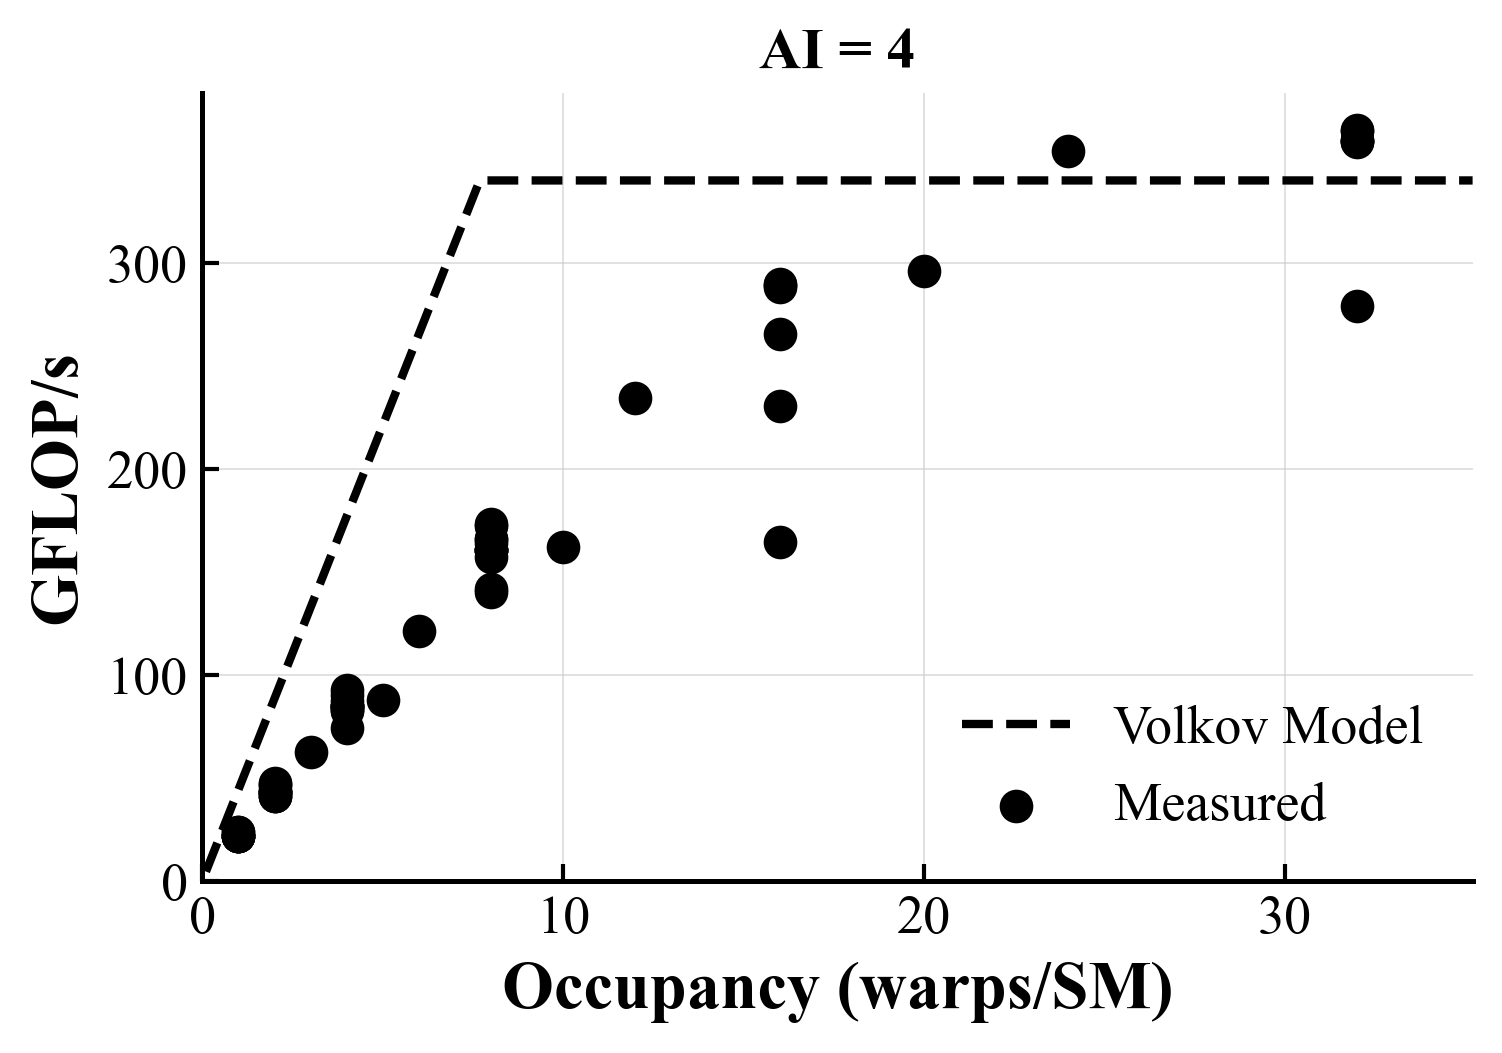
\includegraphics[width=\linewidth]{Results/RTX5000/synthetic_streaming/volkov_rtx5000_a4.png}
  \end{minipage}
  \hfill
  \begin{minipage}{0.32\linewidth}
    \centering
    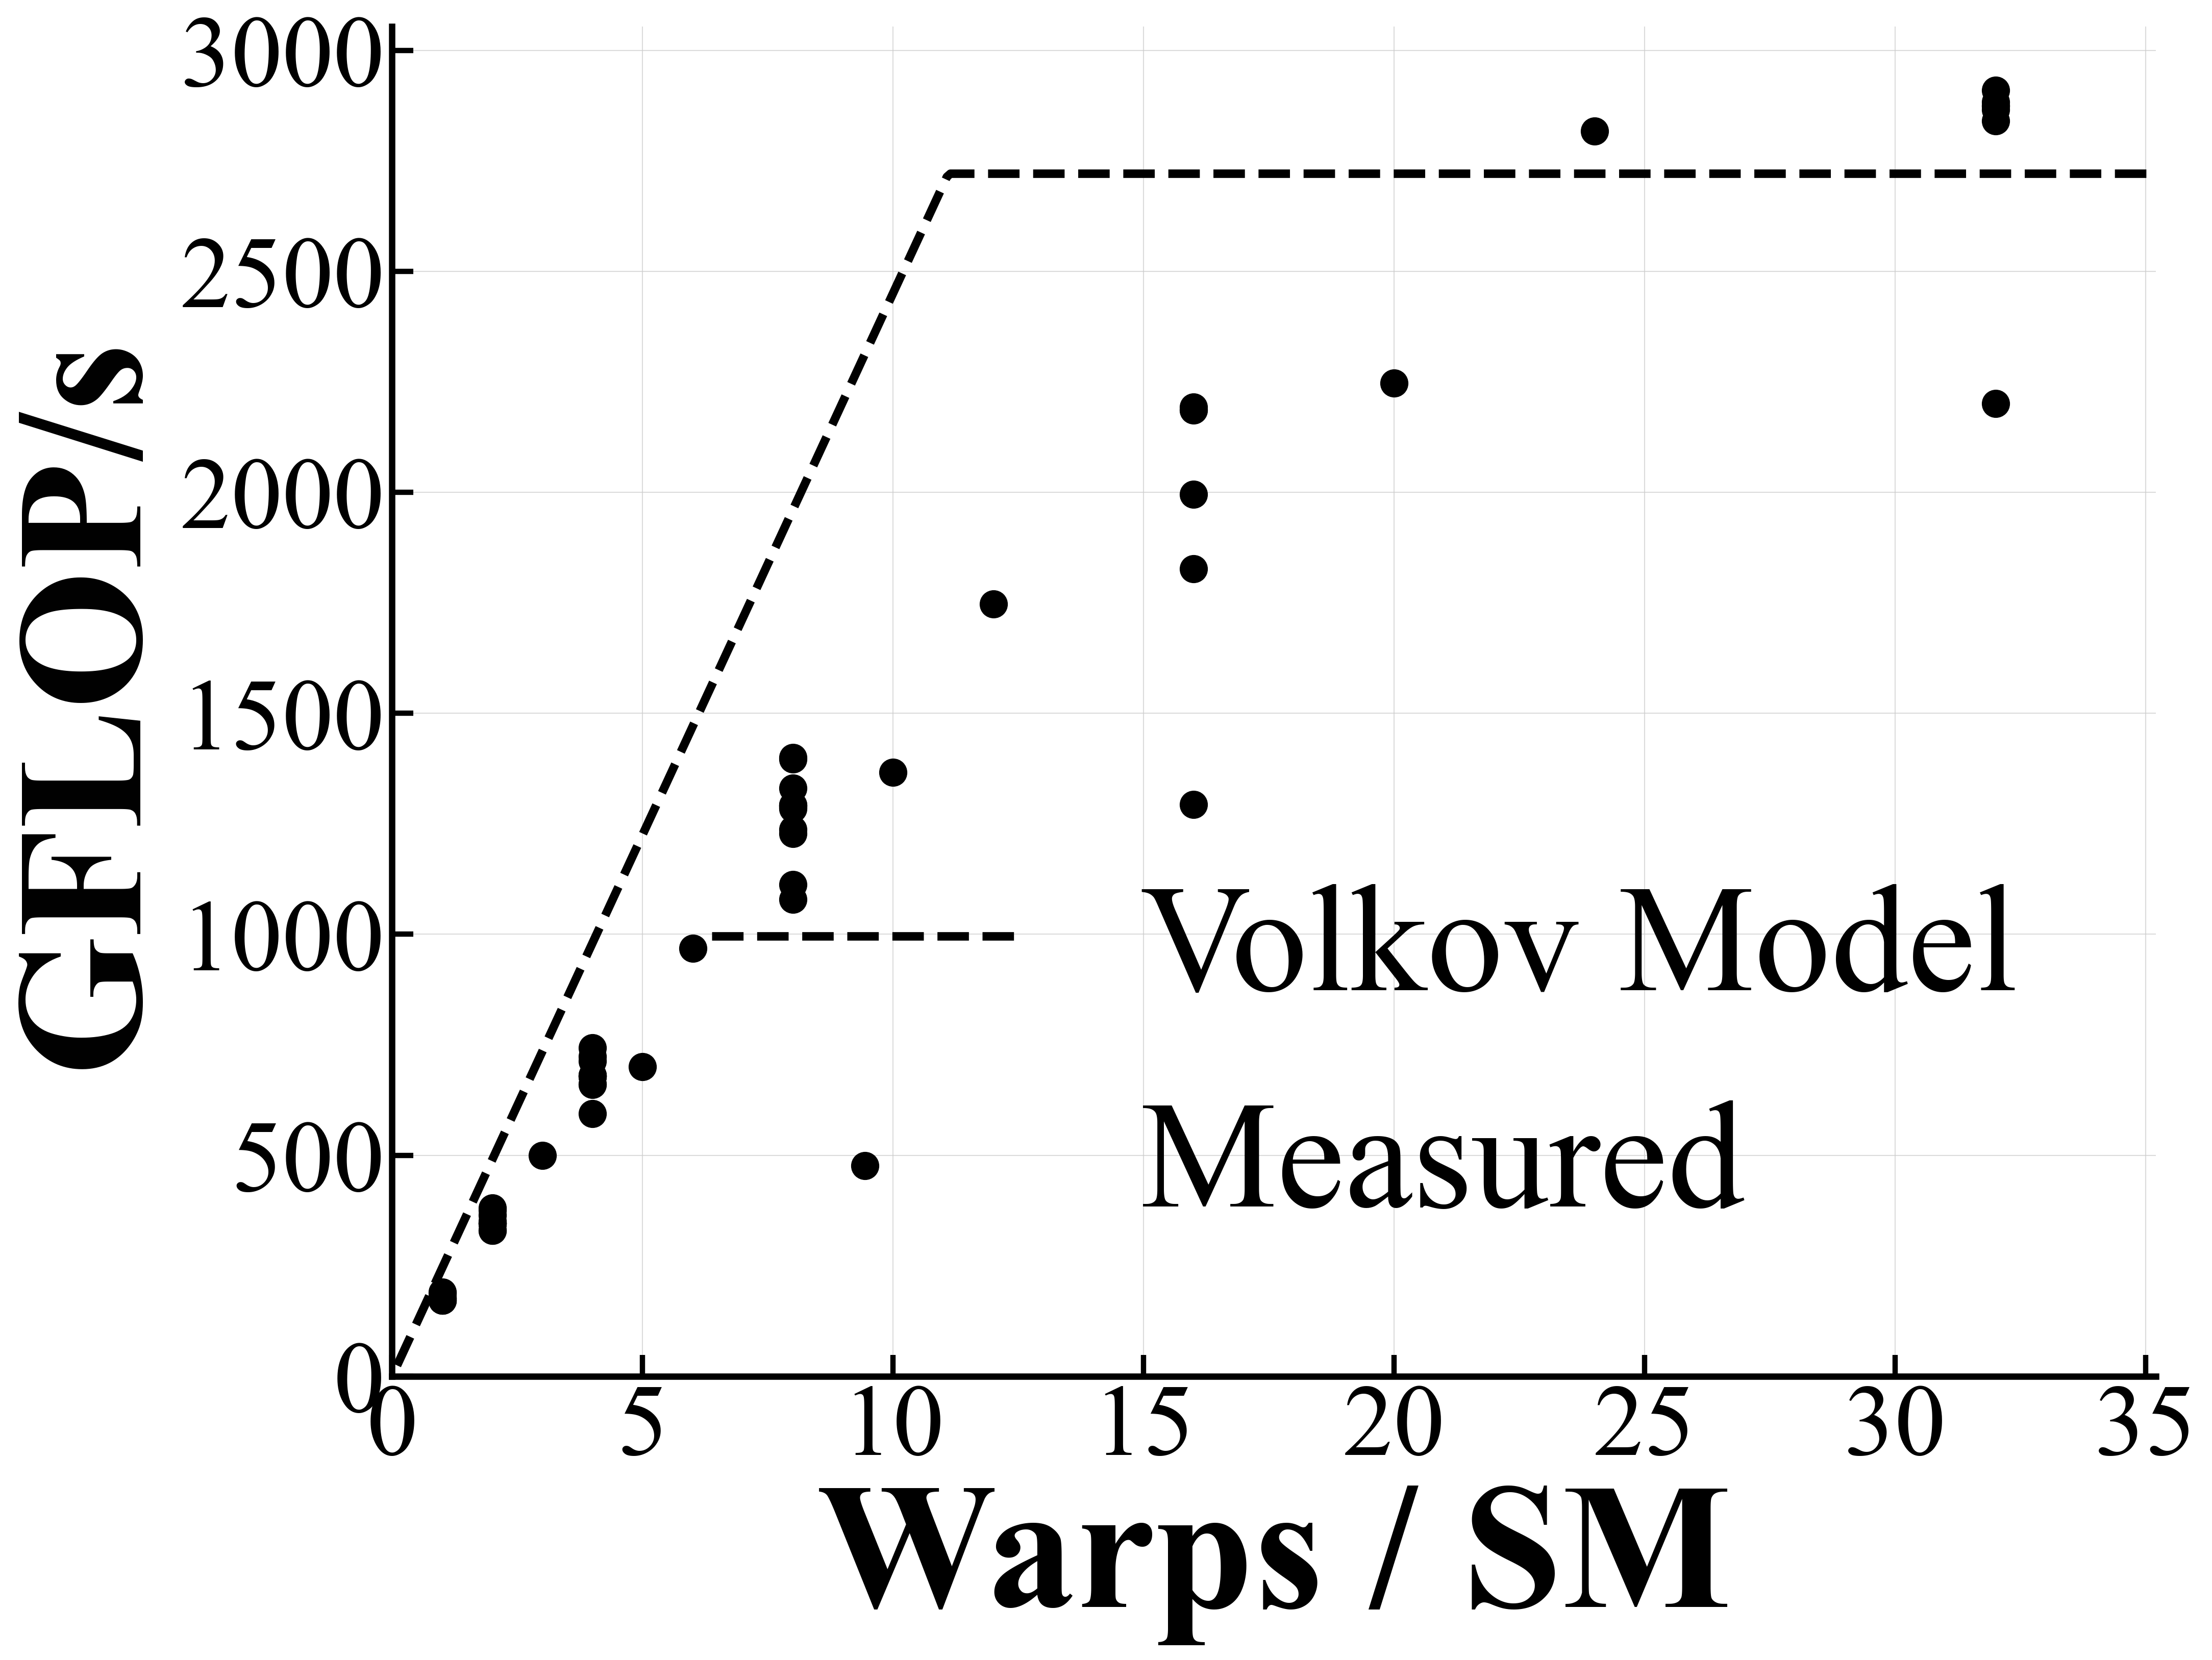
\includegraphics[width=\linewidth]{Results/RTX5000/synthetic_streaming/volkov_rtx5000_a32.png}
  \end{minipage}
  \hfill
  \begin{minipage}{0.32\linewidth}
    \centering
    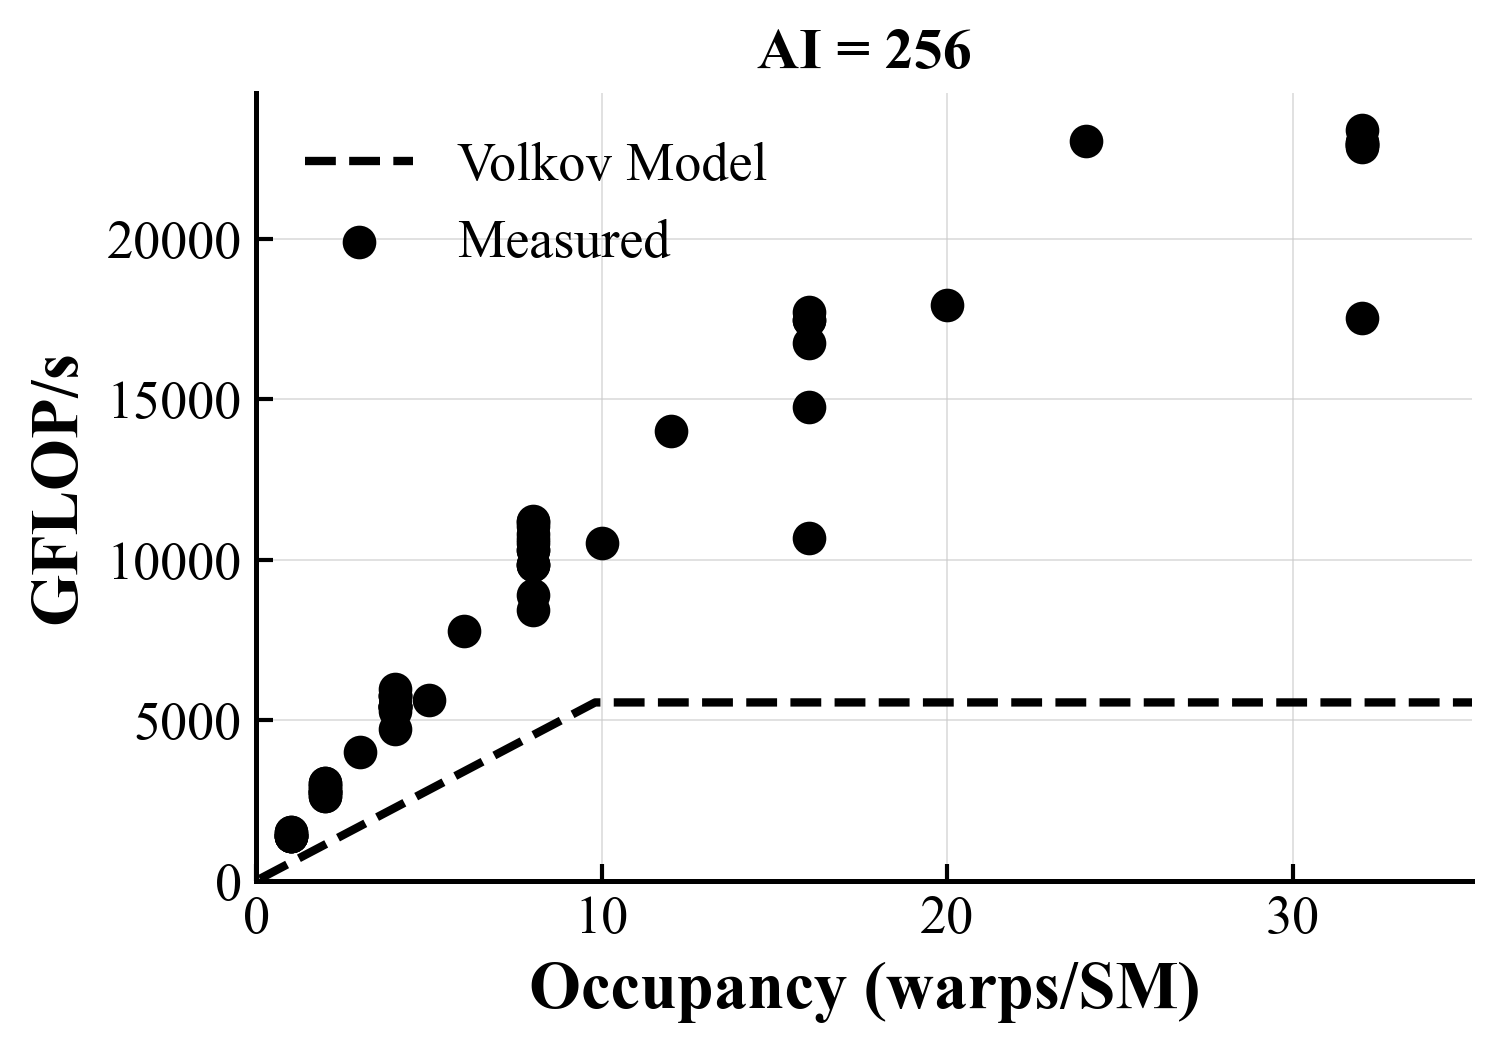
\includegraphics[width=\linewidth]{Results/RTX5000/synthetic_streaming/volkov_rtx5000_a256.png}
  \end{minipage}
  \\[4pt]
  \begin{minipage}{0.32\linewidth}
    \centering
    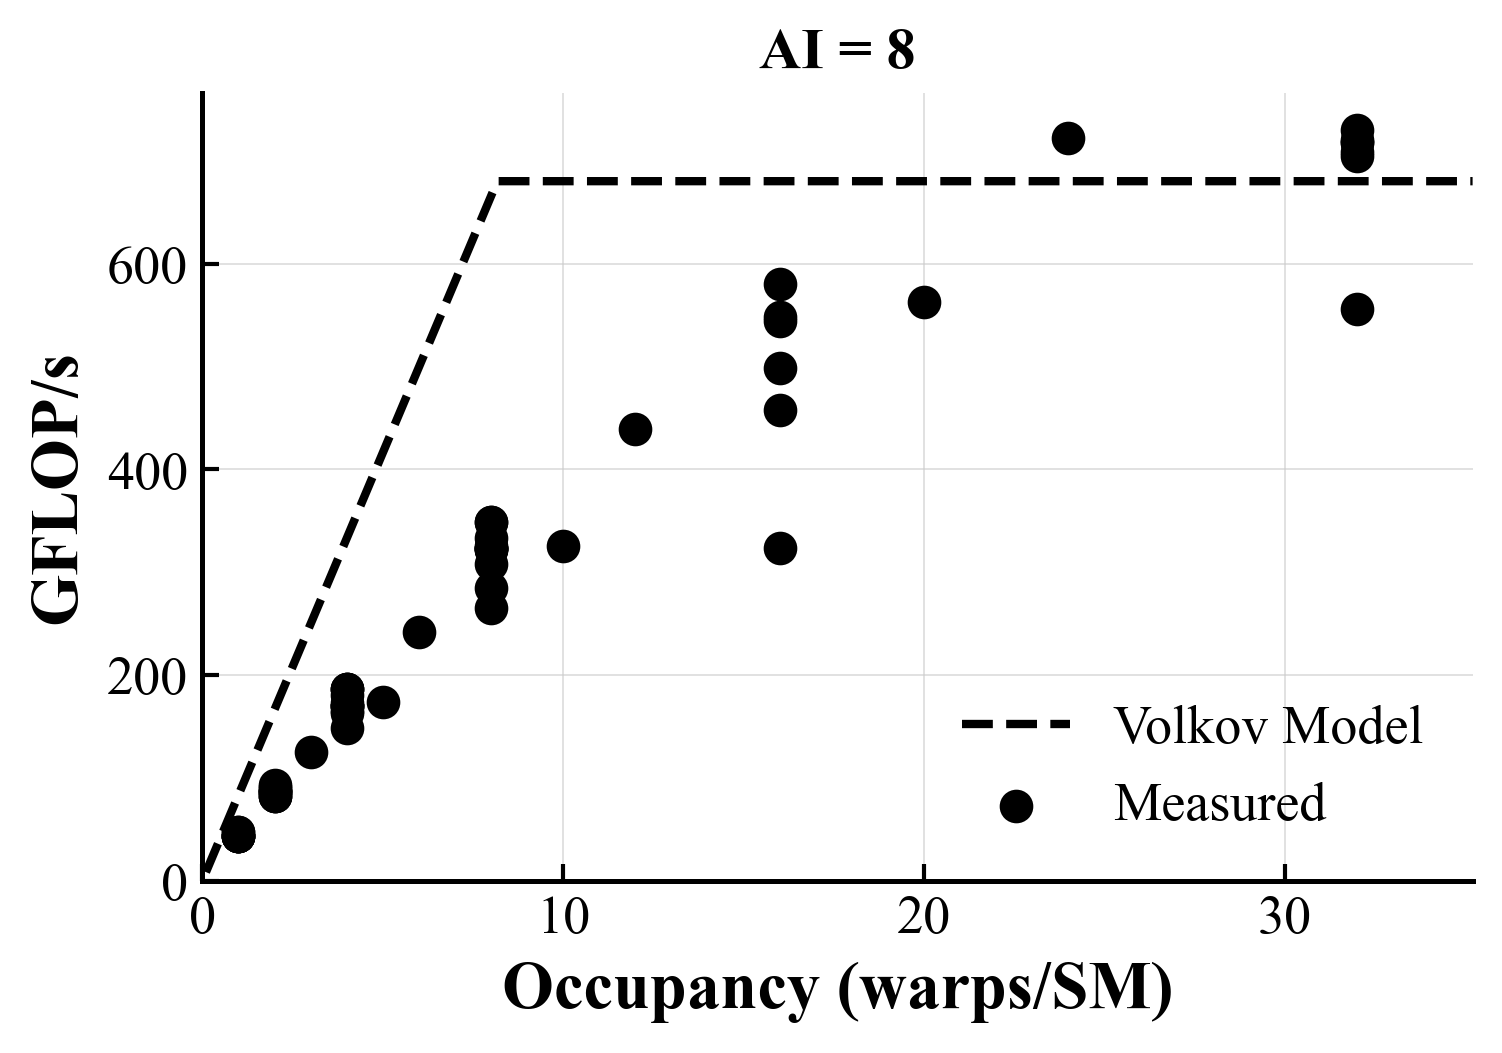
\includegraphics[width=\linewidth]{Results/RTX5000/synthetic_streaming/volkov_rtx5000_a8.png}
  \end{minipage}
  \hfill
  \begin{minipage}{0.32\linewidth}
    \centering
    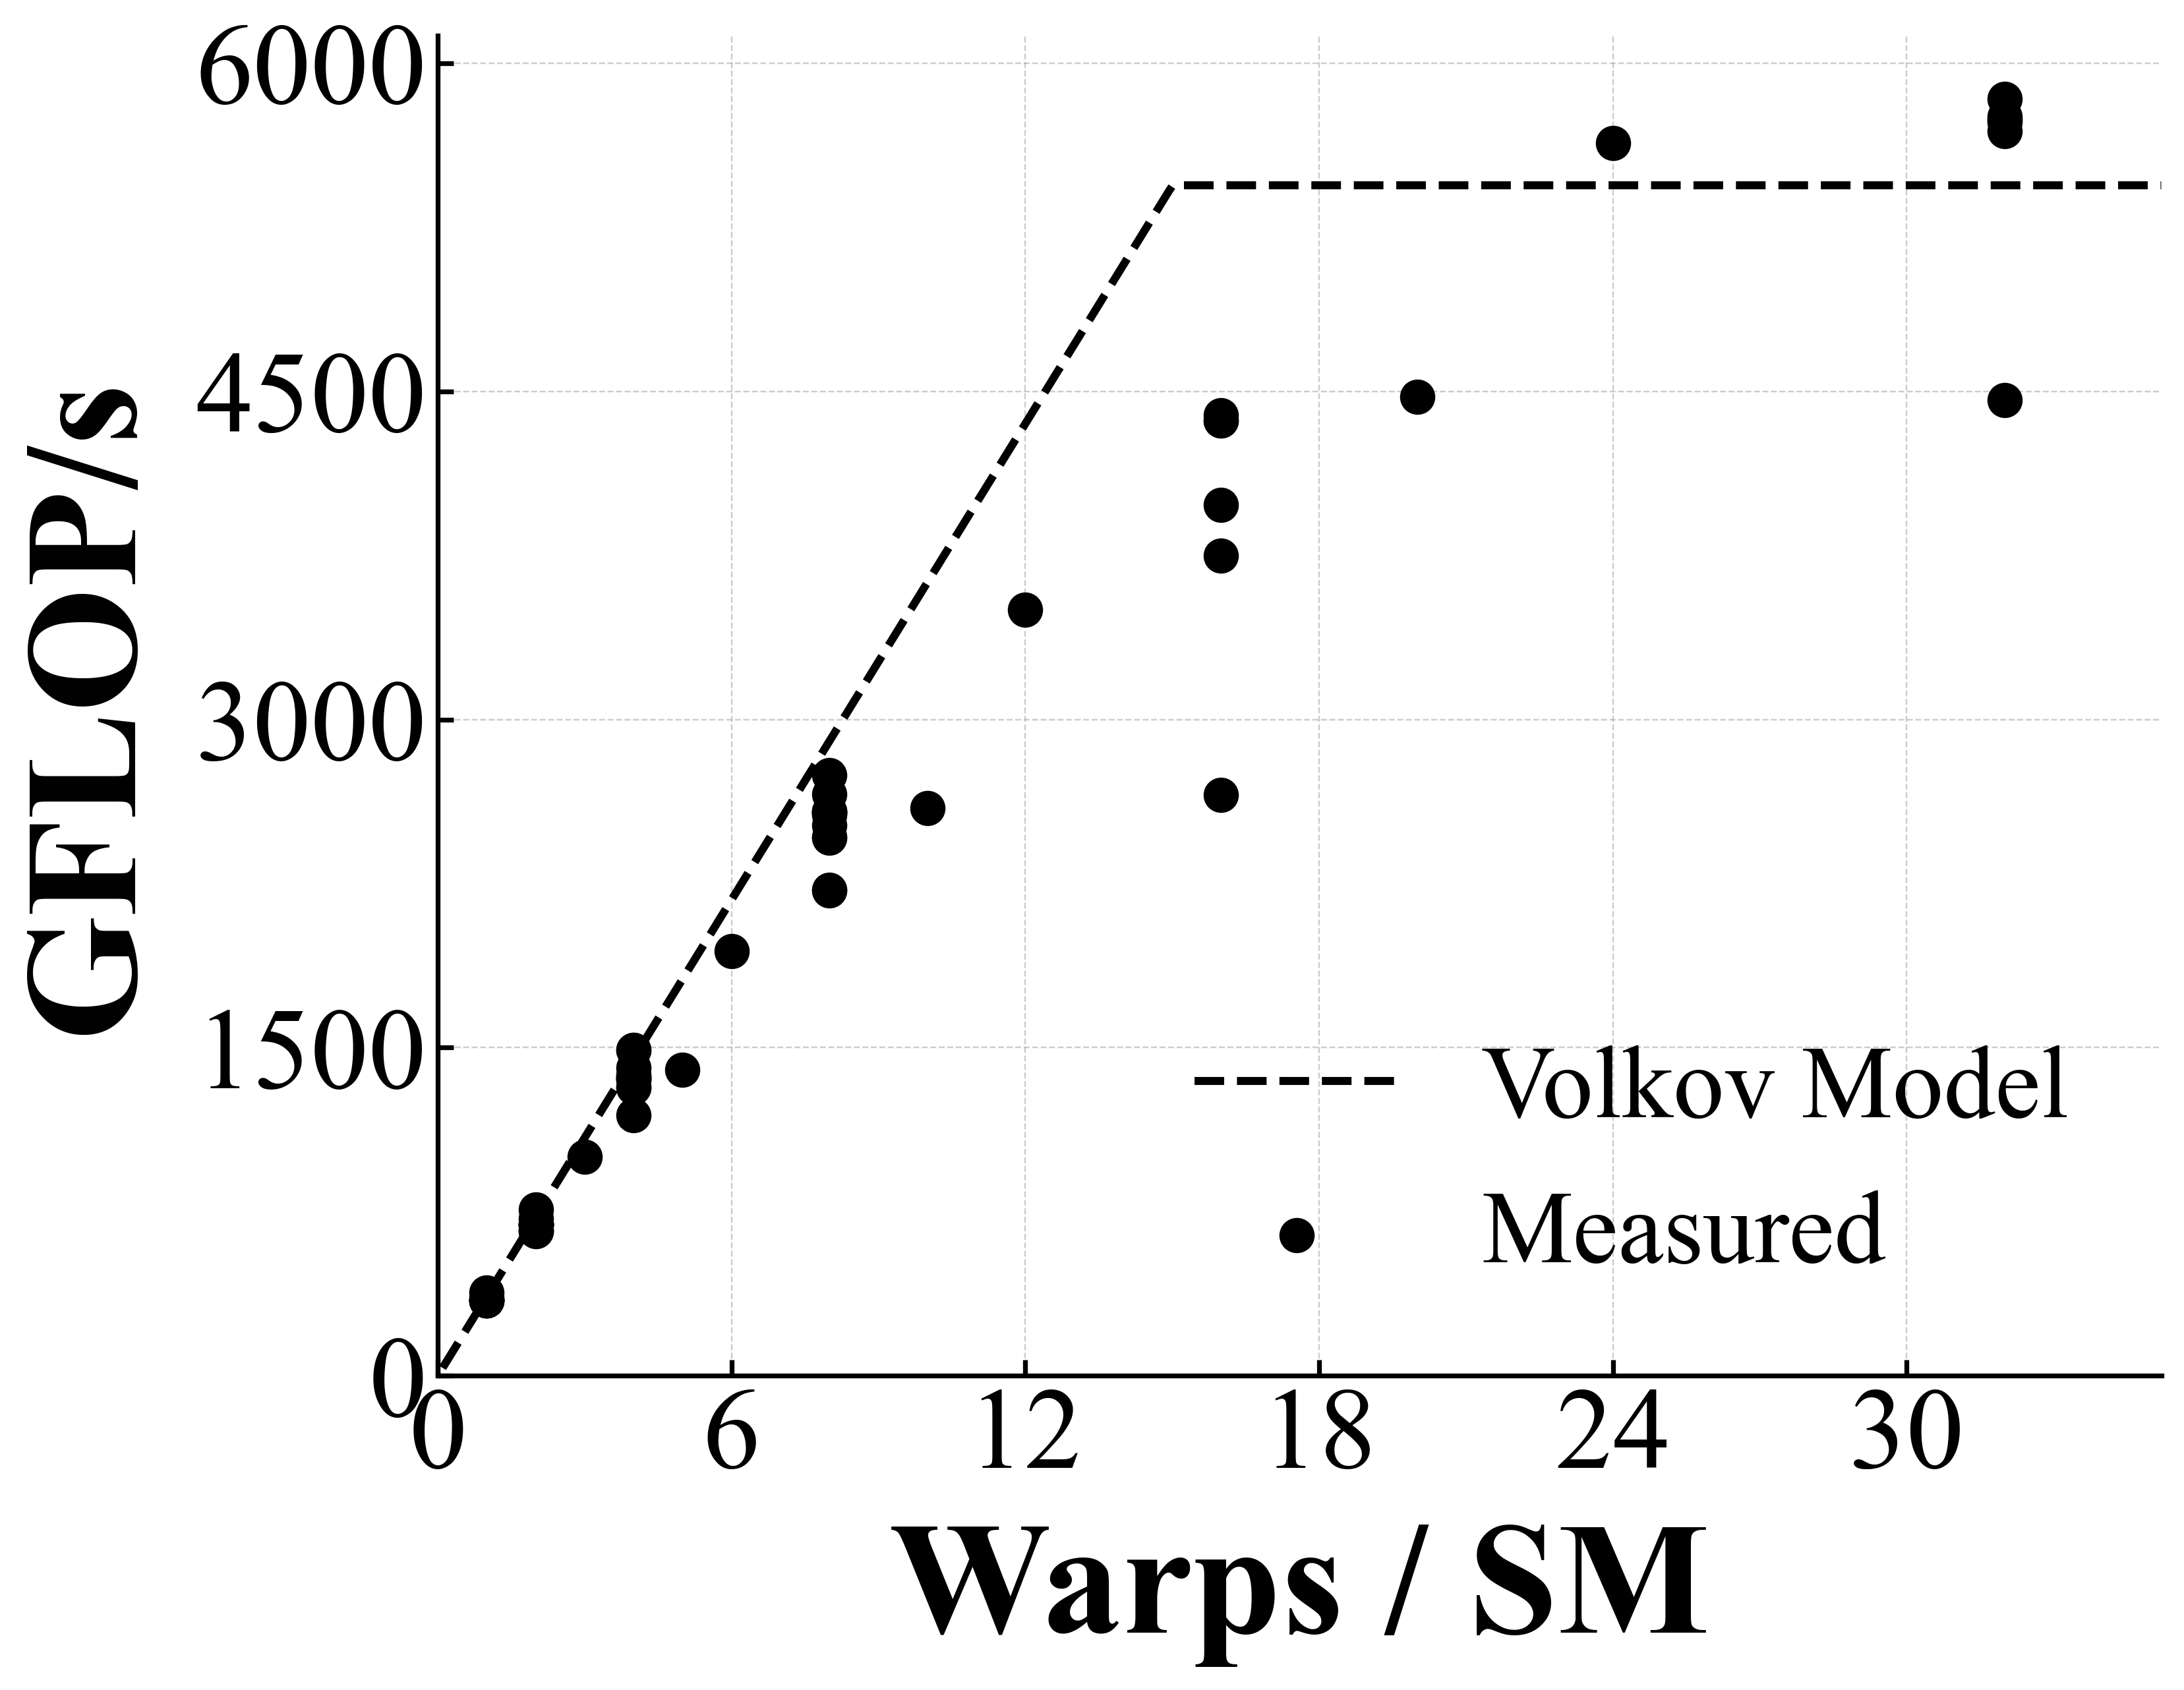
\includegraphics[width=\linewidth]{Results/RTX5000/synthetic_streaming/volkov_rtx5000_a64.png}
  \end{minipage}
  \hfill
  \begin{minipage}{0.32\linewidth}
    \centering
    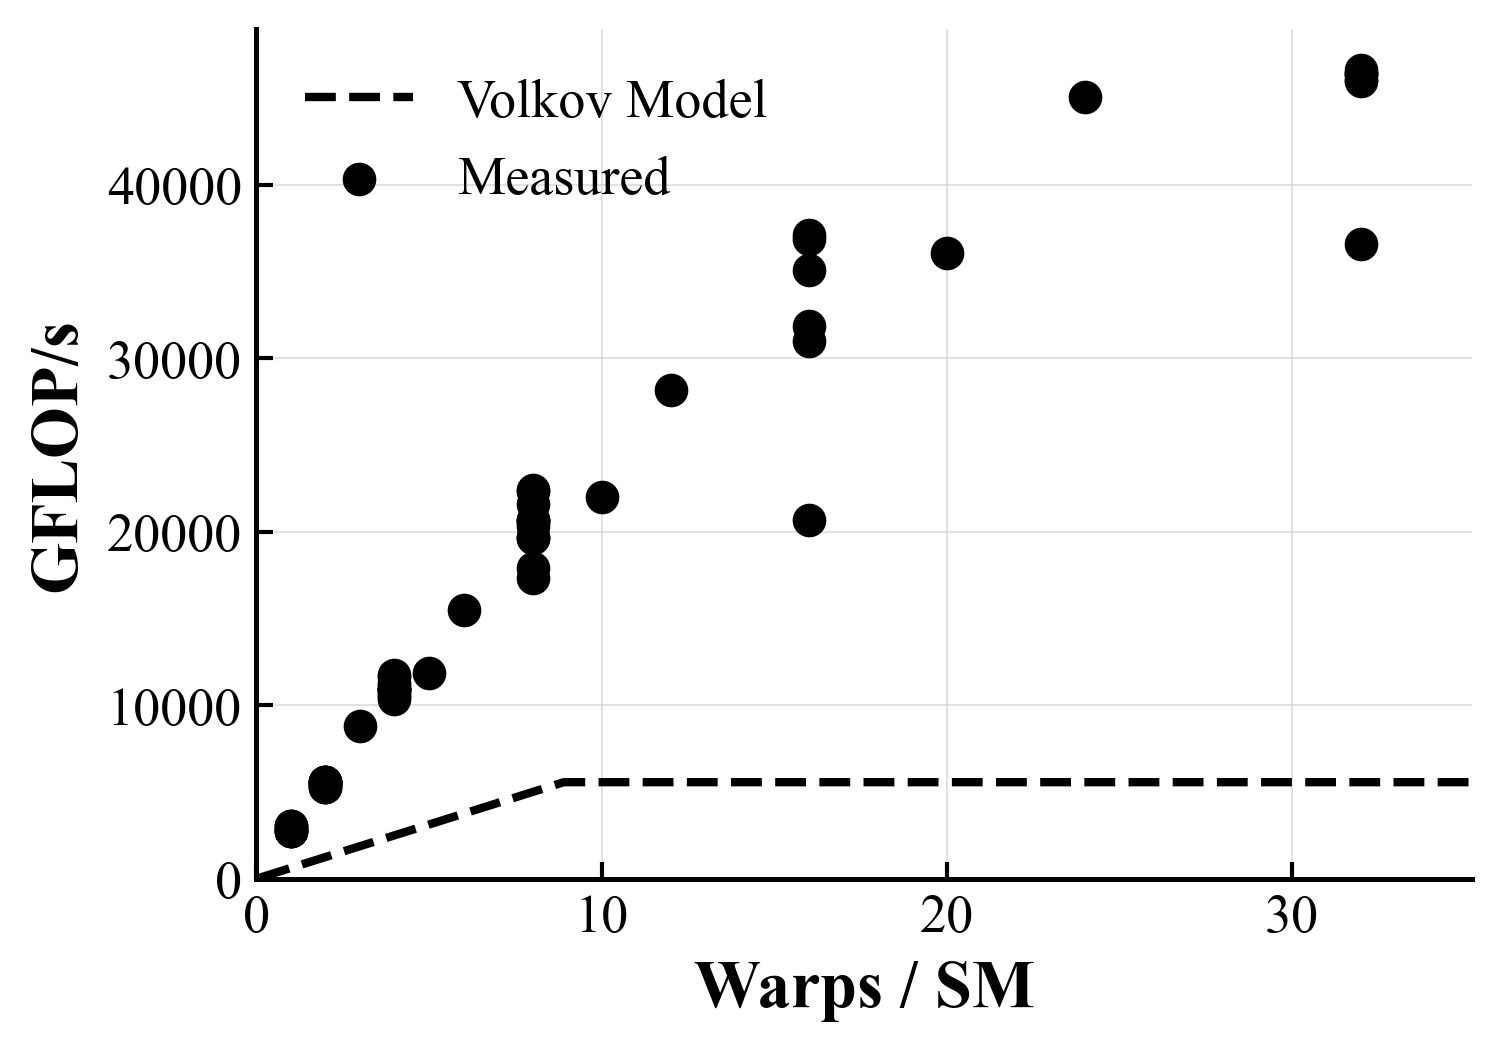
\includegraphics[width=\linewidth]{Results/RTX5000/synthetic_streaming/volkov_rtx5000_a512.png}
  \end{minipage}
  \\[4pt]
  \begin{minipage}{0.32\linewidth}
    \centering
    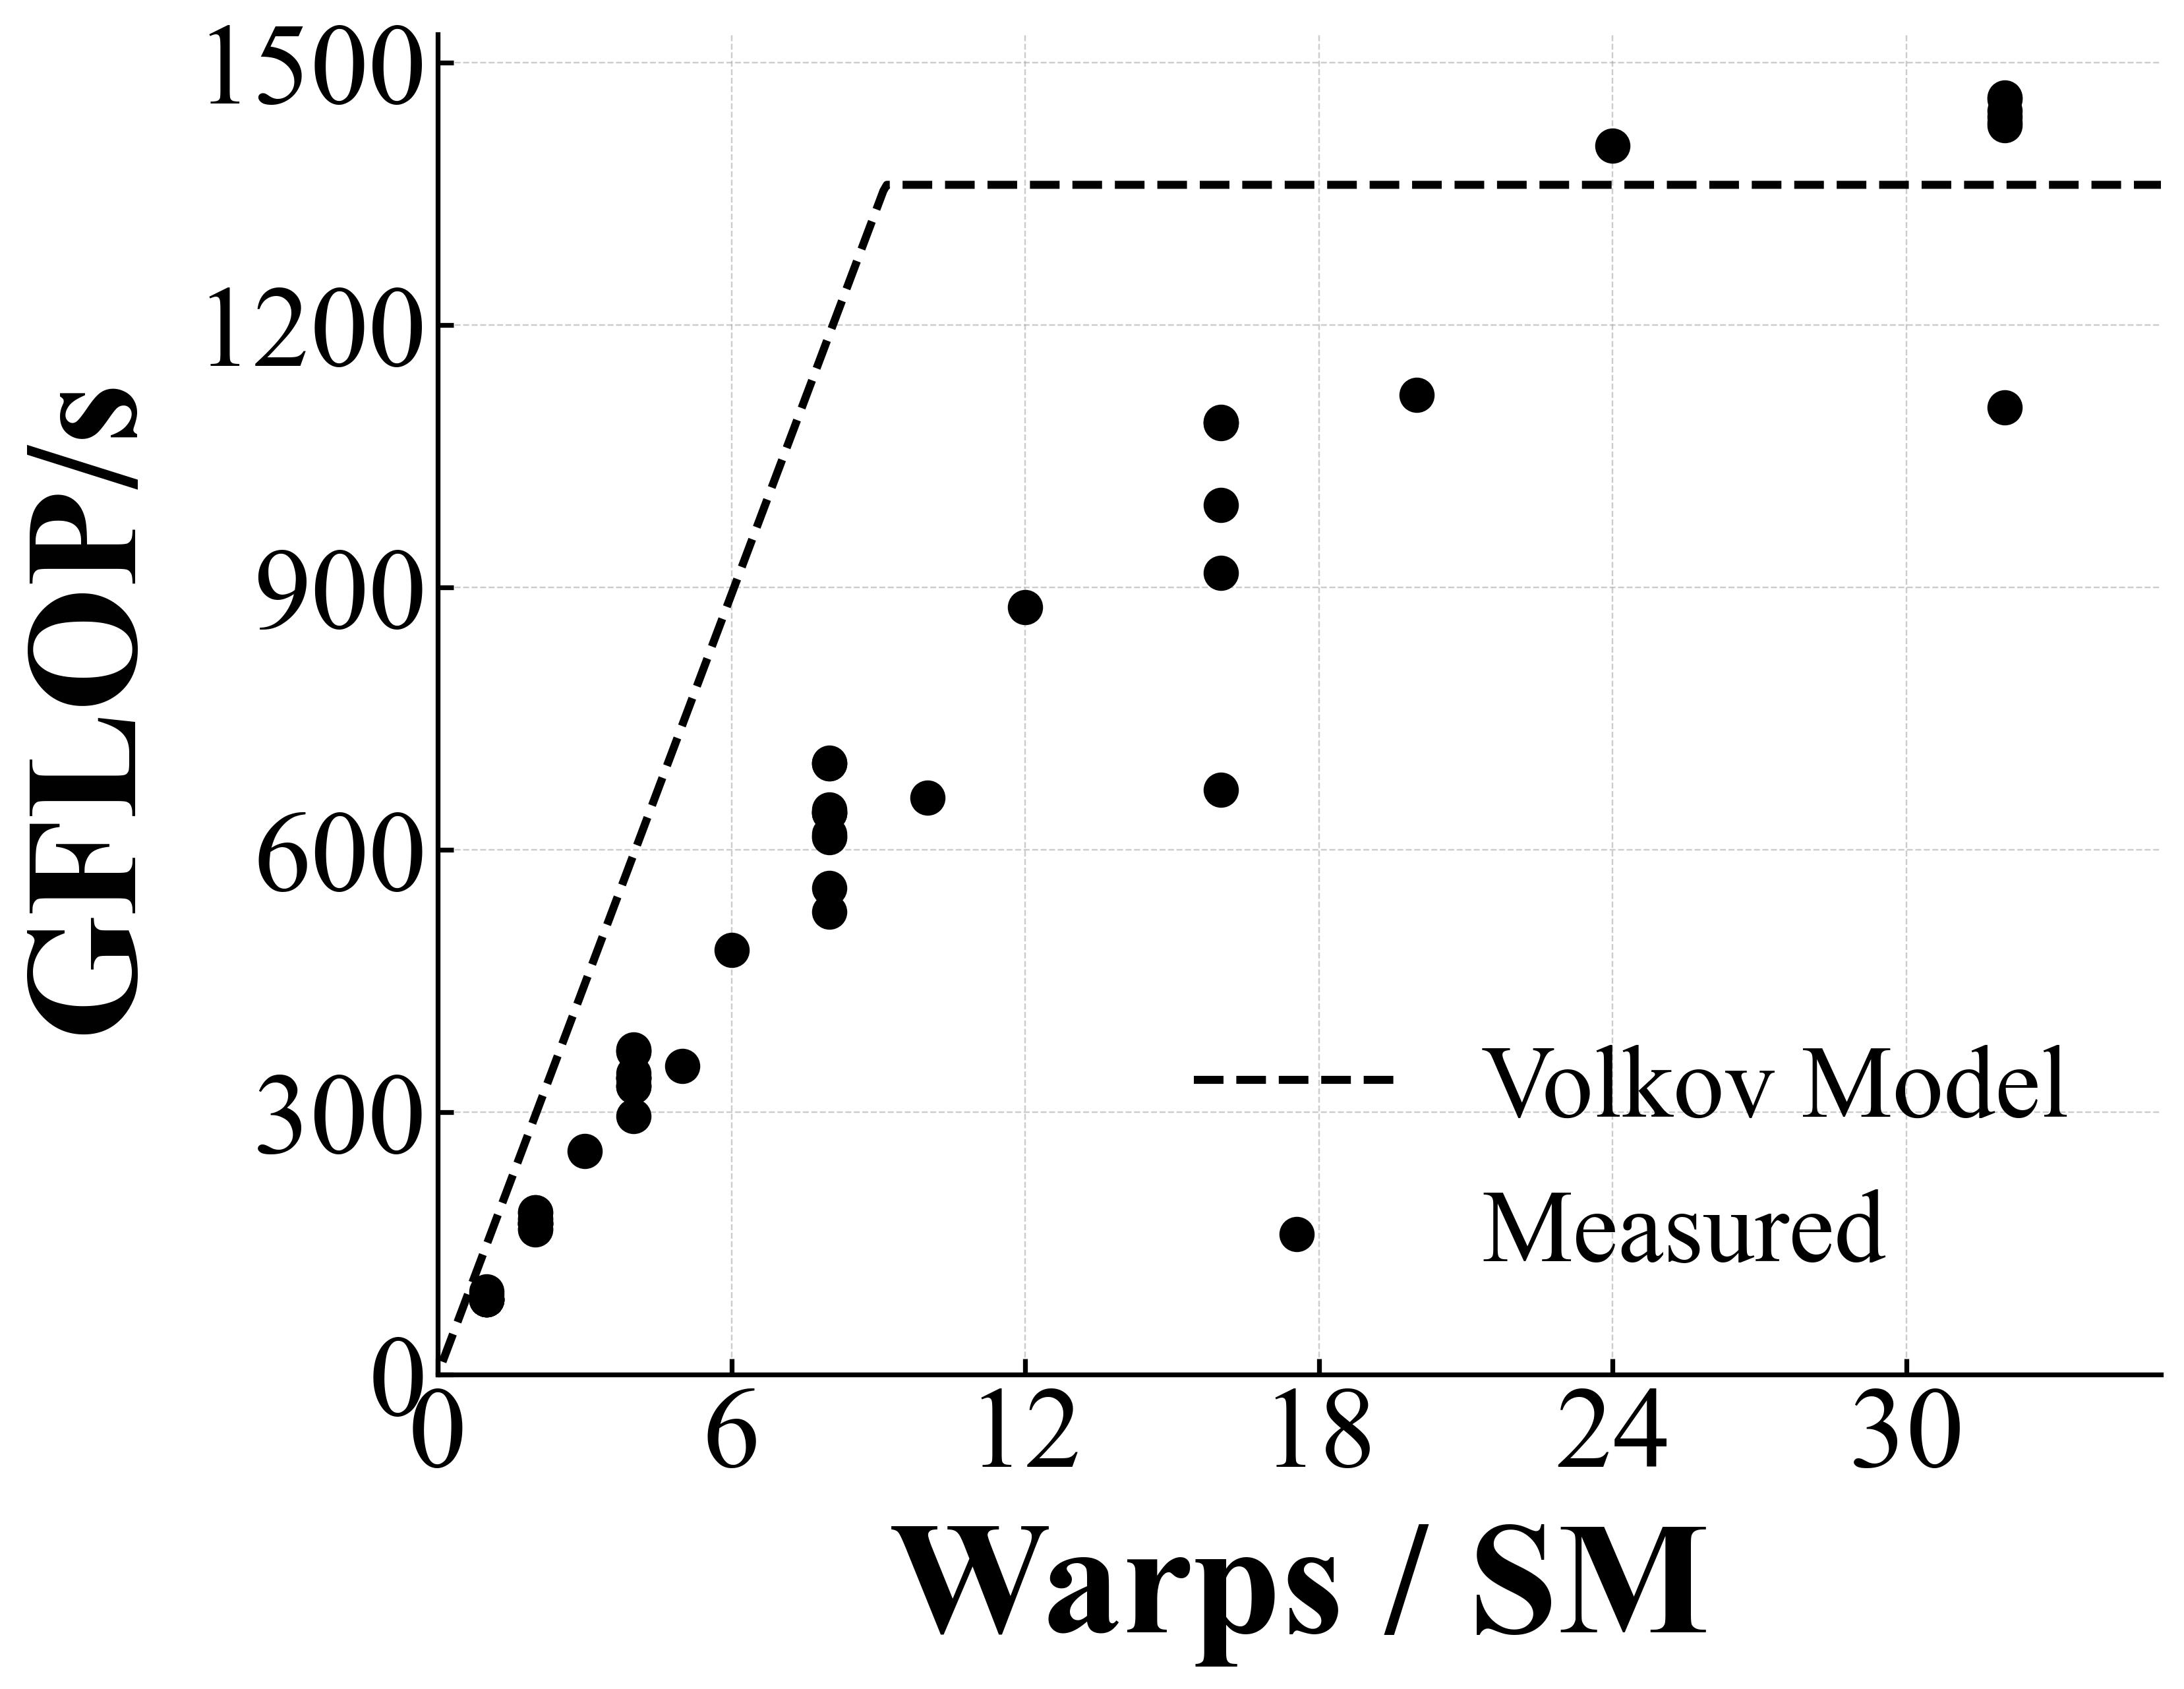
\includegraphics[width=\linewidth]{Results/RTX5000/synthetic_streaming/volkov_rtx5000_a16.png}
  \end{minipage}
  \hfill
  \begin{minipage}{0.32\linewidth}
    \centering
    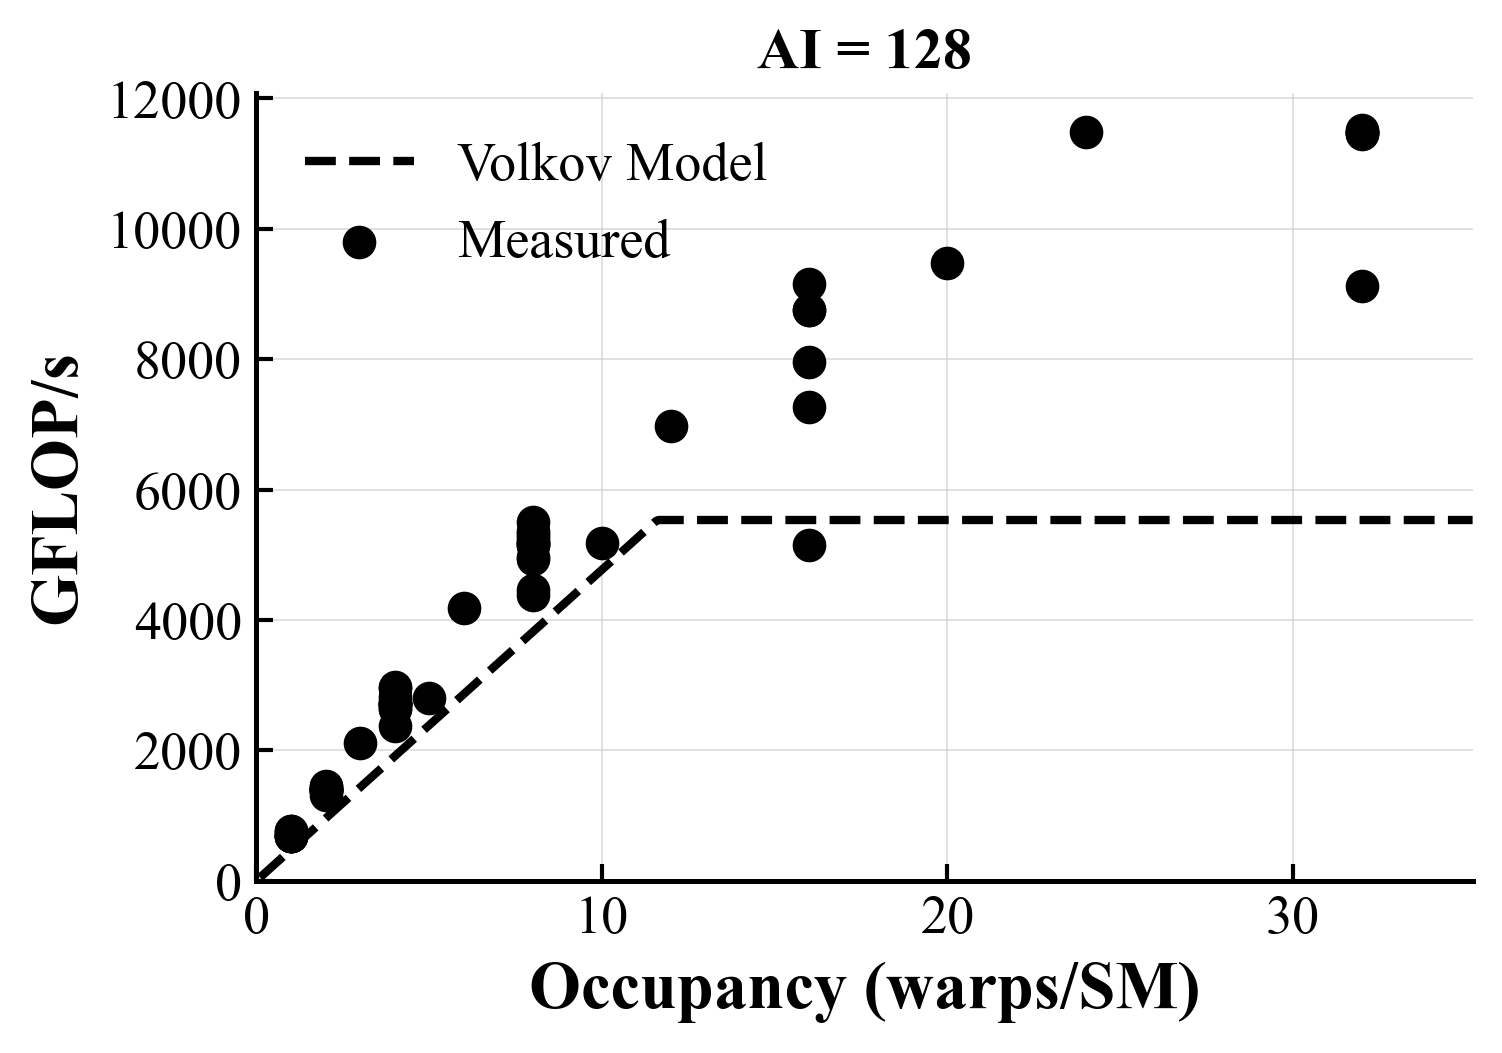
\includegraphics[width=\linewidth]{Results/RTX5000/synthetic_streaming/volkov_rtx5000_a128.png}
  \end{minipage}
  \hfill
  \begin{minipage}{0.32\linewidth}
    \centering
    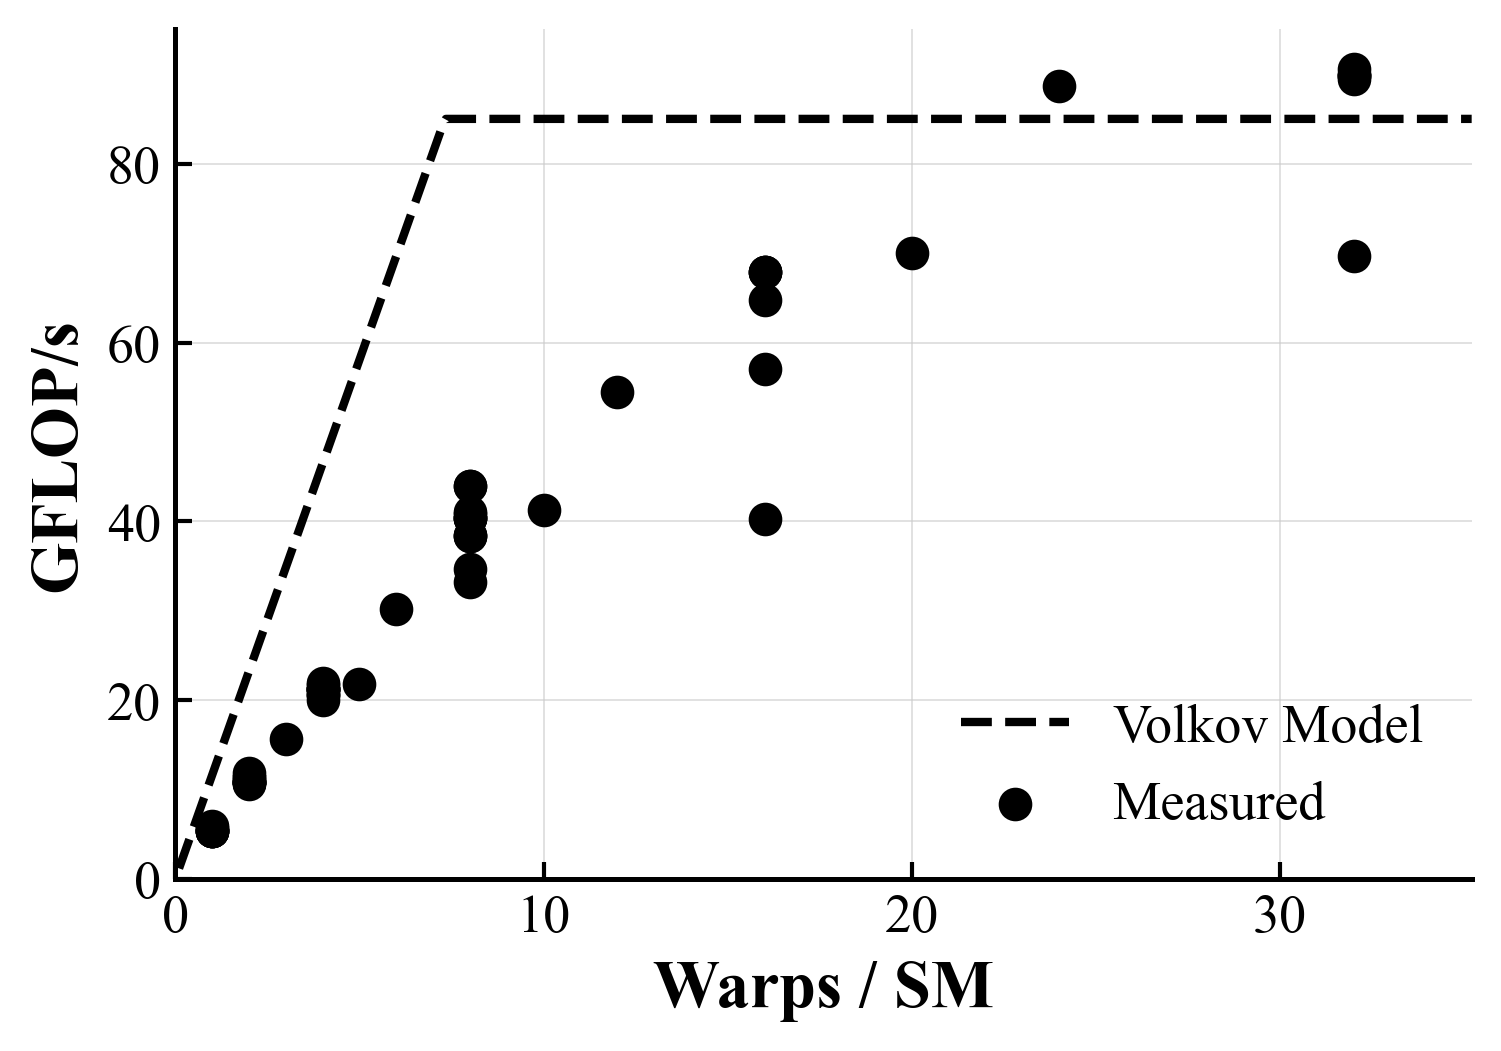
\includegraphics[width=\linewidth]{Results/RTX5000/synthetic_streaming/volkov_rtx5000_a1.png}
  \end{minipage}
  \caption{Volkov model (dashed) vs.\ measured throughput (dots) on RTX\,5000
    for $\alpha \in \{4, 32, 256, 8, 64, 512, 16, 128, 1\}$ (left to right,
    top to bottom).
    The model tracks the data across all arithmetic intensities.
    At low occupancy the latency bound dominates and throughput rises linearly.
    At high occupancy the memory bound or issue bound caps throughput.}
  \label{fig:rtx5000_all}
\end{figure*}

The model tracks measured data well across all $\alpha$ values.
At low $\alpha$ (e.g.\ $\alpha = 1, 2, 4$), the memory bound
($mem_{thru} = 0.0305$) limits throughput early, and the curve plateaus
at a low warps/SM count.
As $\alpha$ grows, more compute instructions fill the time between memory
accesses, and the latency bound shifts to the right: more warps are needed to
reach the memory ceiling.

At high $\alpha$ (e.g.\ $\alpha = 128, 256, 512$), the issue bound
($issue_{thru}/(\alpha+1)$) drops below the memory bound and becomes the
active ceiling.
The model captures this transition correctly.

Table~\ref{tab:rtx5000_peaks} lists the model-predicted and measured peak
GFLOP/s for selected $\alpha$ values.
The error ranges from 2\% to 9\%.

\begin{table}[t]
  \centering
  \caption{Peak GFLOP/s on RTX\,5000: model vs.\ measured.}
  \label{tab:rtx5000_peaks}
  \begin{tabular}{rrrr}
    \toprule
    $\alpha$ & Model & Measured & Error \\
    \midrule
    1   & 85    & 82   & 4\% \\
    4   & 340   & 328  & 4\% \\
    16  & 1360  & 1293 & 5\% \\
    32  & 2720  & 2875 & 5\% \\
    64  & 4181  & 3950 & 6\% \\
    128 & 4322  & 4010 & 8\% \\
    256 & 4348  & 4050 & 7\% \\
    512 & 4361  & 4100 & 6\% \\
    \bottomrule
  \end{tabular}
\end{table}


% ------------------------------------------------------------------
% 5.2  A100 and H100 Results
% ------------------------------------------------------------------
\subsection{A100 and H100 Results}
\label{subsec:a100_h100_results}

% TODO: Fill in once synthetic streaming data is collected on A100 and H100.
% The microbenchmark data is already collected:
%   A100: mem_lat = 240 cycles, alu_lat = 4 cycles
%   H100: mem_lat = 352 cycles, alu_lat = 4 cycles
% What is missing: synthetic_streaming CSV files for A100 and H100.

We apply the same evaluation on A100 and H100.
The model parameters are already measured
(Table~\ref{tab:params}).
The key architectural difference is that H100 has a higher memory latency
(352 vs.\ 240 cycles for A100), which shifts the knee of the latency-bound
curve to the right --- more warps are needed on H100 to reach peak throughput.
H100 also has double the issue throughput ($issue_{thru} = 4.0$ vs.\ 2.0),
so the issue bound is less restrictive.

% Placeholder table --- fill in with actual numbers once available.
\begin{table}[t]
  \centering
  \caption{Peak GFLOP/s comparison across GPUs at selected $\alpha$ values.}
  \label{tab:cross_gpu}
  \begin{tabular}{r|rr|rr|rr}
    \toprule
    & \multicolumn{2}{c|}{\textbf{RTX\,5000}} &
      \multicolumn{2}{c|}{\textbf{A100}} &
      \multicolumn{2}{c}{\textbf{H100}} \\
    $\alpha$ & Model & Meas. & Model & Meas. & Model & Meas. \\
    \midrule
    32  & 2720  & 2875 & ---  & --- & --- & --- \\
    64  & 4181  & 3950 & ---  & --- & --- & --- \\
    128 & 4322  & 4010 & ---  & --- & --- & --- \\
    256 & 4348  & 4050 & ---  & --- & --- & --- \\
    \bottomrule
  \end{tabular}
\end{table}
% TODO: Replace --- with actual A100/H100 data.


% ------------------------------------------------------------------
% 5.3  Comparison with Hong & Kim
% ------------------------------------------------------------------
\subsection{Comparison with Hong \& Kim}
\label{subsec:hk_comparison}

We compare both models across all 10 $\alpha$ values on RTX\,5000
(Figure~\ref{fig:hk_all}).
At low $\alpha$ ($\leq 16$) both models produce similar curves and match the
measured data.
This is expected: when memory latency dominates, the presence or absence of
$alu_{lat}$ makes little difference.

At $\alpha = 32$, the models still mostly agree (Figure~\ref{fig:hk_vs_volkov},
left).
Above $\alpha = 32$, Hong~\&~Kim increasingly overestimates throughput.
At $\alpha = 64$, Hong~\&~Kim predicts roughly $2\times$ the measured peak;
at $\alpha = 128$ and above, the gap grows further.

This confirms the motivation from \S\ref{subsec:hong_kim}: ignoring
$alu_{lat}$ does not matter when memory is the bottleneck, but becomes a
large error source once the arithmetic pipeline depth limits throughput.
Volkov's model, which includes $alu_{lat}$ directly, stays within 2--9\% of
measured values across all $\alpha$ settings.

% Additional Hong & Kim comparison figures (optional -- can use a 2x5 grid)
% \begin{figure*}[t]
%   \centering
%   Include hk_vs_volkov_fixed_a{1..512}.png in a grid here
%   \caption{Hong \& Kim vs. Volkov across all arithmetic intensities.}
%   \label{fig:hk_all}
% \end{figure*}


% ------------------------------------------------------------------
% 5.4  Discussion: Limitations & Generalisability
% ------------------------------------------------------------------
\subsection{Discussion: Limitations \& Generalisability}
\label{subsec:limitations}

Our evaluation uses a synthetic kernel with controlled arithmetic intensity
and coalesced memory access.
This is by design: it isolates the model parameters and allows a clean
comparison.
Real workloads bring additional effects that our evaluation does not cover:

\begin{itemize}
  \item \textbf{Thread divergence.}
    Our kernel has no branches, so all threads in a warp execute the same path.
    Warp divergence would reduce effective throughput in ways that Volkov's
    model does not capture.

  \item \textbf{Shared memory and L1/L2 cache.}
    Our kernel accesses global memory only.
    Programs that use shared memory or benefit from cache hits would see
    lower effective $mem_{lat}$, and the model would need to be initialised
    with the appropriate cached latency.

  \item \textbf{Non-coalesced access patterns.}
    Our streaming kernel uses coalesced loads (128 bytes per warp).
    Random or strided access patterns would require a different $mem_{thru}$
    value and possibly a different $mem_{lat}$.

  \item \textbf{GPU-specific parameters.}
    The four model parameters must be re-measured for each GPU.
    This is quick (the microkernels run in under a minute each) but means
    the model cannot be used off-the-shelf for a new GPU without running
    the benchmarks first.
\end{itemize}

These are not flaws in Volkov's model --- they are boundaries of its scope.
The model is designed for throughput-limited, memory-streaming workloads,
and within that scope it performs well.
Extending it to cache-resident or divergent workloads is left for future work.
